%# -*- coding:utf-8 -*-
%!TEX root = ../thesis.tex

\chapter{水下机器人数学模型搜索与环境识别 }

\label{chap:system_discovery}
% 3.1 引言
% 3.2 系统模型的结构与辨识
% 3.3 基于Levenberg-Marquardt 方法的参数辨识
% 3.4 基于遗传算法的参数辨识
% 3.5 基于符号回归技术的水下机器人模型搜索
% 3.6 基于支持向量机的水下机器人水流环境辨识
% 3.7 小结
\section{引言}

在许多领域的研究中,非线性系统的模型识别是至关重要的\cite{kim2012estimating}。开发的数学模型可以用于研究系统的潜在行为或者对系统进行监督、观测、以及预测系统的发展趋势。此外,数学模型还可以用于控制器,如模型预测控制中。各种系统识别技术被用于动力系统的建模中。

模型的概念已在越来越多的科学领域用来表示观测的系统,而模型的确定就是确定系统在时间中的演化过程\cite{wu2016parametric}。这个过程中,系统受到的力、状态和环境间的相互作用都会被描述。虽然目前的技术进步使得研究者越来越方便地去收集水下机器人的系统测量数据,但是在系统的模型参数化过程仍然受到数据集大小以及数据间的映射关系如模型的数学表达形式的太复杂特点的困扰\cite{menezes2014symbolic,wu2016parametric}。其中有环境的影响,如水流,另外也有噪声等因素的影响作用。
如果使用传统的科学方法,研究人员首先要学习或者建立可以解释水下机器人的数学模型,然后使用测量的数据或者计算方法来分别求解模型中关键项\cite{yang2014modeling,huang2015trends}。然而,
有时研究人员的视角是受到人们固有的知识结构限制,也许模型的表述并不是最好的,而使用者却并不知道。问题在与人们偏爱与寻找能够清楚理解的好模型,而往往直觉确实是不正确的。另外的就是数据测量的运行环境并不能代表系统的所有运行情况,水下机器人的室内水池实验就大多是在静水中的测试,并没有考虑水流等因素。水下机器人系统从环境中获得的信息还很少,并不会主动地辨识环境,这就弱化了水下机器人在水下的生存能力。

水下机器人工作的环境未知多变,使得准确地描述机器人的数学模型并不太容易,其中尤其是非线性水下机器人系统。鱼雷型水下机器人往往比较难以控制,而且多是自主航行,因此要认识它的系统采用以往的方法并不一定可行。水下机器人的非线性的系统模型在上一章中被整理成矩阵形式,但仍需要确定实际系统中应用时的具体结构与参数\cite{garcia2014modelling,Tang2009Estimation,yang2014modeling}。本节将分析REMUS AUV的数学模型,并使用输出状态量与控制输入量,将模型向状态模型的形式变换,从数据驱动的系统建模角度分析水下机器人的模型\cite{brunton2016discovering,schmidt2009distilling}。上一章建立REMUS AUV系统模型,从模型的组成两部分来分析,模型的具体数学表达形式,即模型结构,已经确定。基于此确定的模型结构,仍然需要确定模型中各个参数量,这个过程就是系统辨识\cite{eng2014added}。系统辨识是基于输入和输出的数据以及确定模型形式的系统来确定参数的具体数值。

非线性系统模型的参数辨识已经获得了很大的进展,如本工作中使用的Levenberg-Marquardt算法和遗传算法\cite{baruch2009levenberg,zhou2013genetic}。不过,当所要辨识的目标系统的模型结构未知的时候,这类方法无法正确处理这类AUV系统的模型参数辨识问题。符号回归方法已经成功用于不被了解如何工作的系统的建模,仅仅使用输入输出数据,就可成功地确定出模型的数学表达,并具有难以置信的参数辨识准确率与速度\cite{menezes2014symbolic,Moreno2015Symbolic,wu2016parametric}。不同的是,用符号回归搜索的数学模型,使用基因表达树来表达模型,其本身可以由使用者指定或者自行演化确定。符号回归方法更适合用于搜索模型的数学近似结构,从另一个角度看待系统。

水下机器人工作的深海环境未知性较强,以往的研究给出了航行器受到的主要影响就是水流。深海有多种鱼类生存活动,但是水下机器人的水下工作经常面临不可以预计的危险,主要原因就是其对周围环境的认识能力受限。水下机器人对水下环境的认识能力相比于鱼类感知水环境的能力还相差很远\cite{verschure2003environmentally}。从生物学角度,鱼体侧线器官对水流环境和目标的识别改善了其生存能力。回顾了鱼类对水的感知的一些重要物理结构,特别是侧线系统的感知细胞。在侧线系统的帮助下,鱼可以感知周围的环境,通过感知神经网络受到的刺激信号,将产生神经信号并传输猎物的位置到鱼的大脑\cite{abdulsadda2012artificial,Wu2016lateralline}。神经信号的刺激由侧线系统的生物传感器产生,其中神经丘的机械变形在神经脉冲的表达中转化为压力信号。神经脉冲的处理过程,就是鱼从大量数据中学习水流的模式,可为水下机器人认识水下环境提供参考方法\cite{huang2015trends,martis2013ecg,chen2000new,liu2012support,tagliaferri2015wind}。本章使用获取的水下机器人体周的压力数据,基于数据的稀疏特性将其降维,并使用机器学习方法进行水流方向和速率大小的识别训练与测试,从而让水下机器人更好地认识和利用海洋。

\section{水下机器人模型搜索与参数辨识 }

水下机器人的模型主要包括模型的结构和参数两个主要的部分,本节主要研究非线性6自由度系统模型的水下机器人模型搜索与辨识问题。首先介绍从水下机器人系统中获得的测量数据是如何和系统的模型结构和参数联系起来,分析模型结构已知的辨识方法与未知的方法上的区别。其次是使用Levenberg-Marquardt方法、遗传算法和符号回归方法来对REMUS AUV的模型的参数辨识进行研究,辨识共47个流体动力学参数。最后将对比各个方法辨识水下机器人模型参数的结果,并尝试用符号回归方法搜索用于近似结构的模型,这种近似模型可以用于控制研究。

\subsection{系统模型的结构、参数与系统建模}

在本部分,为了便于后面的系统建模,需要对一个动力学系统的建模问题从黑盒子的角度进行最初的研究。一般要研究的系统会有状态量和输出、输入量。要确定一个系统模型表达,需要收集时间序列的状态数据$\bm{X}$(包括状态量及导数量)。将得到的采样数据写成如下两个矩阵\cite{brunton2016discovering}:
\begin{equation}
\label{eq:chap3:1}
\begin{aligned}
\bm{X} &= \begin{matrix}
\\
\begin{bmatrix}
 \small \bm{X}^T(t_1)     \\
 \small \bm{X}^T(t_2)     \\
 \small \vdots            \\
 \small \bm{X}^T(t_{m})   \\
\end{bmatrix}
 \end{matrix}
= \begin{matrix}
  \rightarrow {state}  \\
  \begin{bmatrix}
   x_1(t_1) & x_2(t_1) & \ldots & x_n(t_1) \\
   x_1(t_2) & x_2(t_2) & \ldots & x_n(t_2) \\
   \vdots   & \vdots   & \ddots & \vdots   \\
   x_1(t_m) & x_2(t_m) & \ldots & x_n(t_m) \\
  \end{bmatrix}
  \downarrow time \\
 \end{matrix}
% \end{equation}
\\
% \begin{equation}
% \label{eq:chap3:2}
\dot {\bm{X}} &=
\begin{bmatrix}
 \small \dot {\bm{X}}^T (t_1)     \\
 \small \dot {\bm{X}}^T(t_2)      \\
 \small \vdots                 \\
 \small \dot {\bm{X}}^T(t_{m}) \\
\end{bmatrix}
= \begin{bmatrix}
   \dot{x_1}(t_1)  &  \dot{x_2}(t_1) & \ldots & \dot{x_n}(t_1) \\
   \dot{x_1}(t_2)  &  \dot{x_2}(t_2) & \ldots & \dot{x_n}(t_2) \\
   \vdots          &  \vdots         & \ddots & \vdots         \\
   \dot{x_1}(t_m)  &  \dot{x_2}(t_m) & \ldots & \dot{x_n}(t_m) \\
  \end{bmatrix}
\end{aligned}
\end{equation}

一个系统的表达主要是有多个不同符号功能组合而成的非线性函数,因此需要选定一个符号功能库,该库包括常数、多项式、三角函数:


\begin{equation}
\label{eq:chap3:3}
\bm{\Theta(\bm{X})}= \begin{bmatrix}
|      & |      &  |         &|           &        &|            &|          &         \\
\bm{1} & \bm{X} & \bm{X}^P_2 & \bm{X}^P_3 & \ldots & sin(\bm{X}) &cos(\bm{X}) & \ldots \\
|      & |      &  |         &|           &        &|            &|          &         \\
\end{bmatrix}
\end{equation}
其中,高阶多项式是就 $\bm{X}^P_2, \bm{X}^P_3$ 等,他们表达的就是模型中非线性功能项。 二次非线性项 $\bm{X}^P_2$ 比表达如下:

\begin{equation}
\label{eq:chap3:4}
\bm{X}^P_2 = \begin{bmatrix}
x_1^2(t_1) &  x_1(t_1)x_2(t_1)   & \ldots & x_2^2(t_1) & \ldots &  x_n^2(t_1) \\
x_1^2(t_2) &  x_1(t_2)x_2(t_2)   & \ldots & x_2^2(t_2) & \ldots &  x_n^2(t_2) \\
\vdots     & \vdots              & \ddots & \vdots     & \ddots & \vdots      \\
x_1^2(t_m) &  x_1(t_m)x_2(t_m)   & \ldots & x_2^2(t_m) & \ldots &  x_n^2(t_m) \\
\end{bmatrix}
\end{equation}

对于水下机器人而言,式\ref{eq:chap3:1}中列就是某个自由度的状态输出量, 要确定水下机器人模型就是求解 $\bm{\Xi}$。
\begin{equation}
\label{eq:chap3:5}
\dot{\bm{X}} =
\bm{\Theta}(\bm{X}) \bm{\Xi}
\end{equation}
其中 $\bm{\Xi} = [\bm{\xi}_1, \bm{\xi}_2,\ldots,\bm{\xi}_n]$ 是系数矩阵。

一般在系统辨识中采用辨识方法多是基于最小二乘法的\cite{friedman2001elements},需要写出系统模型的目标函数,就需要对式\ref{eq:chap3:5}进行变换,从而更加利于辨识的执行。给出的目标函数的形式如下\cite{brunton2016discovering,wu2016parametric}:
\begin{equation}
\label{eq:chap3:6}
\dot{\bm{X}}_k = \bm{f}_k(\bm{X}) = \bm{\Theta}(\bm{X}^T)\bm{\xi}_k
\end{equation}
\begin{equation}
\label{eq:chap3:7}
\dot{\bm{X}}= {\bm{\Xi} }^T (\bm{\Theta}(\bm{X}^T))^T
\end{equation}

水下机器人的动力学系统也可表达成状态方程的形式,因此水下机器人的系统参数也可以使用基于最小二乘法的辨识方法\cite{baruch2009levenberg}。不过这种辨识方法是有个前提,即式\ref{eq:chap3:6}中的用于描述符号功能的块是必须已经确定。本章提出的符号回归方法可以同时对模型的结构部分与参数部分进行进化,并使用性能评判函数筛选最佳估计值。下面分别介绍Levenberg-Marquardt算法、遗传算法和符号回归算法用于参数辨识的例子。此外也使用符号回归算法搜索了模型结构未知时候的可能最佳近似模型。

\subsection{基于Levenberg-Marquardt方法的参数辨识 }

 Levenberg-Marquardt(LM)方法是对求取目标函数最小值的高斯牛顿方法一种受欢迎的替代选择,该方法具有高斯牛顿方法和梯度下降方法的两者优点,是一种有效的广义非线性最小二乘法算法\cite{baruch2009levenberg}。REMUS AUV 的动力学模型是非线性的,表达形式可以写成$y=f(x,\theta)$ 的形式,其中$x$ 是函数变量, $\theta$ 是需要识别的参数,水下机器人的最小二乘法问题可以定义为如下形式:

\begin{equation}
\label{eq:chap3:7}
F\left( \theta  \right) = \frac{1}{2}\sum\limits_{i = 1}^m {{{\left[ {{y_i} - f\left( {{x_i},\theta } \right)} \right]}^2}}
\end{equation}
式中,$y_i$ 是模型的估计值,$f(x_i,\theta)$ 是实际系统的值。辨识的过程就是求解式\ref{eq:chap3:7}的最小值的过程。

当平方和函数,$ F(\theta)$,为最小值时,平方和函数相对 $\theta$ 的梯度是为0的。由 $f(x_i,\theta+\delta)$ 的一阶近似可以给出如下平方和函数:

\begin{equation}
\label{eq:chap3:8}
{\rm{F}}(\theta  + \delta ) \approx \sum\limits_{i = 1}^m {{{\left( {{y_i} - f\left( {{x_i},\theta } \right) - {J_i}\delta } \right)}^2}}
\end{equation}

求出平方和函数相对于 $\delta$ 的导数形式,并令导数为0,则可以得到

\begin{equation}
\label{eq:chap3:9}
\left( {{J^T}J} \right)\delta  = {J^T}\left[ {y - f\left( \theta  \right)} \right]
\end{equation}
其中,$J$ 是第 $i$ 行等于 $J_i$ 的雅可比矩阵,其中$f$ 和 $y$ 分别是具有第 $i$ 个分量 $f(x_i,\theta)$ 和 $y_i$的向量。

Levenberg-Marquardt方法使用搜索方法来求出线性方程组的解,它通过使用“阻尼项”代替方程\ref{eq:chap3:9}的对应项,可以得到新得
\begin{equation}
\label{eq:chap3:10}
\left( {{J^T}J + \lambda I} \right)\delta  = {J^T}\left[ {y - f\left( \theta  \right)} \right]
\end{equation}
其中,\textit{I}是单位矩阵,并给出被估计参数向量的增量 $
\delta$,非负标量 $\lambda$ 是用来控制增量的步长和方向。


\subsection{基于遗传算法的参数辨识  }

遗传算法(GA)是一种模拟生物进化过程中的自然选择机制而求解问题的全局优化方法。对于水下机器人的非线性水动力学参数的辨识问题,一群个体组成的解的集合是基于适应度函数的评估不断进化以便选出最好的参数估计解\cite{yuan2010genetic,zhou2013genetic,chang2007nonlinear}。

适应度函数对于保持解的精度非常重要,本文将输出误差的加权值作为适应度函数来进行评估。如此,可以将参数辨识问题转变成为遗传算法的参数优化问题。

水下机器人的适应度函数定义如下:
\begin{equation}
\label{eq:chap3:11}
{J_j} = \sum\limits_{i = 1}^m {\left| {\frac{{{X_j}(i) - {{\hat X}_j}(i)}}{{{X_j}\left( i \right)}}} \right|}
\end{equation}
其中,$X=[u,v,w,p,q,r]$ 是水下机器人在体坐标系的状态向量,$X_j$ 是 $X$ 的第 $j$ 个量。

遗传算法的基本优化流程如下:\\
步骤1:随机生成群体,设置最大代数,以及其他终止条件。\\
步骤2:个体评估:计算种群 $P(t)$ 中每个个体的适应度函数。\\
步骤3:选择操作:根据适应度值对当前种群 $P(t)$ 应用选择操作。\\
步骤4:交叉操作:将交叉操作应用于种群 $P(t)$ 以产生下一代。\\
步骤5:突变操作:将变异操作应用于种群 $P(t)$ 。\\
在步骤3,步骤4,步骤5之后,根据所有的个体的适应度函数值可以得到下一代种群 $P(t)$ 。\\
步骤6:终止条件判断:如果 $t = T$ 满足其他终止条件,则处理中具有最合适适应度函数值的个体将被选为辨识问题的最优解。 否则,回到步骤2。\\

\subsection{基于符号回归技术的水下机器人模型搜索  }

\subsubsection{符号回归 }

回归分析是研究科学问题的基本方法之一。回归的任务是辨识输入变量 $x = [x_1, x_2,\ldots,x_j]$ 和 数据中不断变化的因变量 $y = [y_1, y_2, \ldots,y_k]$之间的数学关系。其中, $j$ 是每个观察值中的自变量的标号,$k$ 是因变量的标号。建立的数学关系为了确定自变量和因变量之间的映射关系,并测试搜索到的模型的质量和一般性。在回归过程中,辨识是从确定一个不确定的数学映射关系函数到识别一个预定义的目标函数的参数值。然而这意味着,参数可以由辨识方法自动的调节,而目标函数的结构必须由一个人类专家定义才可以。符号回归是一种基于遗传技术的用来搜索表达空间以减少多种评价函数误差量的回归方法\cite{schmidt2009distilling}。

符号回归可以估计水下机器人系统模型的参数并可同时改善方程式的结构表达。然而,传统的线性和非线性回归方法只能通过辨识具有预定方程结构的观测系统模型的参数值。虽然其他很多方法都可以辨识模型的参数值,但是符号回归方法因为可以对模型的数学表达式的结构上做操作,而优势明显。符号回归方法的主要思想是集中于搜索目标空间的可能解上,而放弃一些不大有希望的数学解空间。符号回归算法是通过模仿遗传和进化算法的机理来完成搜索任务的。符号回归中运算操作主要有突变、交叉、选择,这些都可以用来处理模型的代数数学表达式的进化。虽然机理来源相同,但是在具体的处理技术上有些差异,表达解的方法是多种多样\cite{dos2009nonlinear,Gandomi2012A1}。遗传编程是一个由生物自然演化启发的进化算法, 其中使用非正式和正式符号来改善模型的结构表达,以及提高大量数据处理应用中的计算效率,如符号回归。

在REMUS AUV模型的回归处理中,一个水下机器人模型的初始表达式由数据随机地从一群符号表达方程中选择出来。每一次进化中,通过重新组合以前的模型表达式,并使用交叉和突变处理以产生新的表达形式,这些解的个体会构成一个新的种群。每次进化得到的种群都和上一代的种群不相同。在每次选择处理中,对REMUS的数据建模比较好的模型会被存储下来。基因和编码被用来表达REMUS的数学模型的符号形式,以便于进行回归处理。如此,该方法将可以发现模型数据中最可能的数学表达方程,并可以用来解释隐藏在水下机器人观测数据中内在关系。

\subsubsection{遗传编程 }

遗传编程(GP)是一种符号优化技术,它使用基于达尔文自然选择原理创建计算机程序来解决给定的任务\cite{schmidt2009distilling,dos2014genetic,feng2006identification,garg2014mathematical}。 遗传编程和遗传算法之间的差异在于对问题解的表达方法不同。遗传算法中,以字符形式的数字被创建出来以表达解,而遗传编程中,通常使用树结构的形式来表达各个解,并将这些解构成一个计算程序的一部分。与遗传算法一样,遗传编程技术也是在全局范围内进行搜索的,并极力避免陷入到局部最优解的搜索困境,但是由于对于问题表达的规范性更强,操作处理更加准确。

正如符号回归部分所述,水下机器人系统建模的方程式的个体构成的群体随机地被创建出来以获得搜索解的多样性。群体中的每个成员都是一个包括功能集和数据变量集的分层结构树。表达个体的数据集和功能集是从程序预先设定的功能和变量集中选择出来的。例如,运算功能集中的函数表达F会包括基本代数运算操作符号(+, - ,*,/等等)、布尔逻辑函数(AND,OR,NOT等)或任何其他数学函数。变量数据集T则包含函数中各种参数,可以有数字常量、逻辑常数、变量等构成。函数中运算功能集和变量集中的各个元素被算法挑选出来组合在一起以获得水下机器人模型示例的基因型结构染色体表达,其中REMUS的某个自由度运动的数学方程包括功能和变量均会被存储为二进制的形式。图\ref{fig:chap3:F1}中示出了用于航行器偏航运动的简化方程\ref{eq:chap3:12}的GP模型的基因树表示的模型示例。

\begin{equation}
\label{eq:chap3:12}
 I\dot r = {N_{\dot v}}\dot v + {N_{\dot r}}\dot r + {N_v}v + {N_r}r + {N_{uu\delta }}{u^2}\delta
\end{equation}

\begin{figure}[!htp]
  \centering
  \includegraphics[width=14cm]{figure/chap3/gptrees.png}
  \label{fig:chap3:F1}
  \bicaption[fig:chap3:F1]{GP树表示的REMUS偏航方程}{GP树表示的REMUS偏航方程} {Fig.}{GP trees for the Yaw motion of REMUS(see equation(\ref{eq:chap3:12})) }
\end{figure}


遗传编程的初始种群的创建是在可能的解决方案的大空间中盲目搜索的一个可能的解决方案。一旦模型群体被随机创建出来,遗传编程方法将会开始评估种群的每个个体,并选择部份个体进行繁殖操作,并使用突变、交叉以及直接繁殖操作以产生新的个体。最后,在每次迭代中不断地创造出新的个体,并优化产生新群体\cite{Gandomi2012A2,stoutemyer2013can}。

交叉操作时,随机地选择每个解个体(程序)基因树的分支上的一个点,然后交换每个程序的变量集或功能集,这样可以创建出两个新程序个体(见图\ref{fig:chap3:F2})。在进化过程的每次迭代中,使用适应度函数值评估新群体,并开始新一轮的繁殖和交叉操作。在遗传编程算法的这个过程中,从模型中选择一个变量或功能符号,并使用变异操作(见图\ref{fig:chap3:F2})。在任何一代出现的最好的程序个体,以及至今最好的解个体,定义了遗传编程算法的输出\cite{Gandomi2012A1,schmidt2010symbolic}。

\begin{figure}[!htp]
\centering
\includegraphics[width=14cm]{figure/chap3/GPevolution.png}
\label{fig:chap3:F2}
\bicaption[fig:chap3:F2]{遗传编程进化过程示意}{遗传编程进化过程示意} {Fig.}{Schematic of automatic evolution of Yaw motion equation using GP }
\end{figure}

根据计算返回的误差度量值,在进化的每个回归过程中,REMUS AUV的偏航运动模型的数学表达式将被预测和评估性能。虽然机器人的模型中包含非线性项(例如,$sin$,$cos$),但是遗传编程算法的运算可以用二进制编译方法将新形式的方程个体创建出来。在每一代的回归过程中,可以给出目标方程的具体表达,并可以从中确定流体力学系数的参数数值。根据提出的误差标准,符号回归获得的运动模型的质量好坏可以被检查和评估。因此,可以从训练数据中轻松地获得REMUS AUV的模型结构和系数。符号回归的求解过程比Levenberg-Marquardt算法和遗传算法等最小二乘法更为方便,计算甚至更准确。搜索REMUS模型的结构和参数表明,基于遗传编程技术的符号回归方法可以成功应用于水下机器人非线性模型的识别。

\subsection{结果与分析 }

本节将介绍Levenberg-Marquardt算法,遗传算法和符号回归方法的辨识水动力参数的估计结果,并使用符号回归方法搜索测量数据集以发现AUV模型的新形式。

A. 误差评估

使用符号回归、Levenberg-Marquardt方法、遗传算法对实验数据辨识的结果可以使用误差直接评估。 为了检查使用的辨识方法的性能,将计算平均绝对误差(MAE),均方误差(MSE)和混合相关/误差(HCE)。  MAE,MSE和HCE计算公式如下:

平均绝对误差(Mean Absolute Error):
\begin{equation}
MAE = \frac{1}{N}\sum\limits_{i = 1}^N {\left| {y - f\left( x \right)} \right|}
\label{eq:chap3:mae}
\end{equation}
假设噪声服从双指数分布,可以使用MAE缩小残差的绝对值。

均方误差(Mean Squared Error):
\begin{equation}
MSE = \frac{1}{N}\sum\limits_{i = 1}^N {{{\left( {y - f\left( x \right)} \right)}^2}}
\label{eq:chap3:mse}
\end{equation}
假设误差噪声服从正态分布,使用其可以缩笑均方残差值。

混合相关误差(Hybrid Correlation/Error):
\begin{equation}
HCE = \sum\limits_{}^{} {\sum\limits_{}^{} {\left( {\sum\nolimits_{X,Y} {} } \right)} }  + \frac{1}{N}\sum\limits_{i = 1}^N {\left| {y - f\left( x \right)} \right|}
\label{eq:chap3:hce}
\end{equation}
式中,将相关性和绝对误差进行组合。

在上面公式中,$y$ 是输出值, $f(x)$ 是目标值, $N$ 是测量的总数。MAE, MSE对于三个算法都适用,而HCE仅仅用于符号回归到评估中。

B. 初始设置与预处理

考虑到过程噪声对航行器模型系统的影响,REMUS模型的数值实验和参数识别是基于方程\ref{eq:chap2:30}和各个自由度的非线性方程\ref{eq:chap2:surgeremus}、\ref{eq:chap2:swayremus}、\ref{eq:chap2:heaveremus}、\ref{eq:chap2:rollremus}、\ref{eq:chap2:pitchremus}与\ref{eq:chap2:yawremus}进行的。测量的运动数据包括大量的噪声,水下航行器系统的非线性模型中的噪声通常被认为是高斯白噪声,假定为零均值高斯白噪声且是相互独立的\cite{sabet2014extended}。本文中用于航行器的建模参数估计的运动数据中包含的噪声被进行了预处理以加快了寻找最优解解的搜索速度和可能性。数据的预处理包括几个选项:平滑数据,处理缺失值,移除异常值,归一化比例和偏移以及应用过滤器。在应用预处理于测量数据集的搜索过程之后,也可以使用可以找到目标函数的全局最优值的参数优化函数来进一步消除噪声的影响。为了验证噪声对搜索过程的影响,已经使用几种不同信噪比(SNR)传感器模型处理在不同初始条件下进行的数值模拟实验中测量的运动数据,并基于REMUS运动动力学方程对各种参数进行识别。

Levenberg-Marquardt(LM),遗传算法(GA)和符号回归(SR)都是全参数回归估计方法,可以识别连续时间序列运动数据的流体动力学参数。 此外,基于符号回归的识别还可以用于估计质量不高的数据集的模型参数,尤其是其中一段时间的数据(时段)丢失或随机组合的一系列测量数据。 因此,符号回归更灵活,可以获得更好地识别系统模型。

为了对比应用于水下机器人REMUS AUV 系统模型的参数识别方法的整体性能,通过设定不同的航行速度从 $u = 0.5$ 设置为 $u = 3m/s$,控制面舵转向角从-20 到 20度。 其中,当前进速度 $u$ 的速度为 $2 m/s$ 时,可得到 AUV 的 3-D 运行轨迹,如图\ref{fig:chap3:F3}所示,其中控制面板舵和升降角均为10度。 初始条件是所有粘性系数均为零。 此外,分别使用SNR = 1, 10, 20, 45 的传感器模型来测量状态变量的值。

\begin{figure}[!htp]
\centering
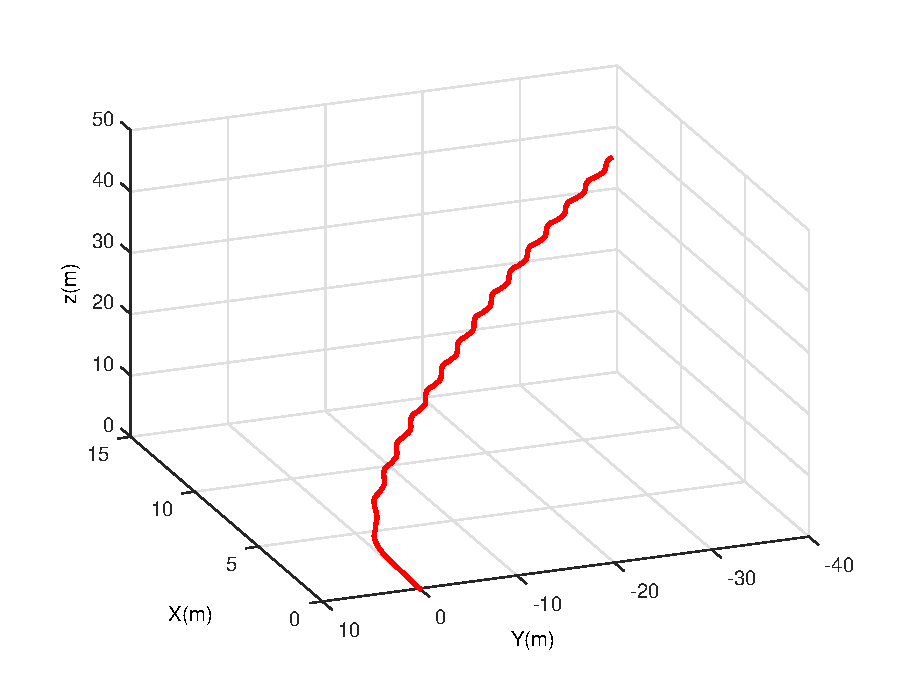
\includegraphics[width=10cm]{figure/chap3/trajectory_anlge_10_u_2.eps}
\label{fig:chap3:F3}
\bicaption[fig:chap3:F3]{AUV的3D运行轨迹}{AUV的3D运行轨迹} {Fig.}{AUV's trajectory on 3-D plot}
\end{figure}

从数值实验获得的测量数据是每个自由度中AUV的速度值。 然而,目标函数是从REMUS AUV的数学模型中推到出的,其包含符号回归中实用的加速度。 为了提高计算速度和便于搜索最优解,使用方程\ref{eq:chap3:13}中描述的欧拉数值方法来获取每个时刻加速度值。 此外,在实际测量中获得的数据主要是速度或加速度的状态数据的一部分,这对于参数辨识并不够。 也可以通过适当地使用欧拉数值方法获得所有必要的状态数据以方便进行参数辨识。

\begin{equation}
\begin{array}{l}
\label{eq:chap3:13}
 \dot u\left( k \right) = \left[ {u\left( {k + 1} \right) - u\left( k \right)} \right]/h \\
 \dot v\left( k \right) = \left[ {v\left( {k + 1} \right) - v\left( k \right)} \right]/h \\
 \dot w\left( k \right) = \left[ {w\left( {k + 1} \right) - w\left( k \right)} \right]/h \\
 \dot p\left( k \right) = \left[ {p\left( {k + 1} \right) - p\left( k \right)} \right]/h \\
 \dot q\left( k \right) = \left[ {p\left( {k + 1} \right) - p\left( k \right)} \right]/h \\
 \dot r\left( k \right) = \left[ {r\left( {k + 1} \right) - r\left( k \right)} \right]/h \\
 \end{array}
 \end{equation}
其中, $h$ 是采样的时间间隔。

使用Levenberg-Marquardt方法来估计具有已知非线性结构的水下机器人模型的参数。 方法是使用MATLAB中使用优化工具箱实现的,LM方法的设置条件如下:TolFun为1e-8,迭代最大次数为800,每个参数的上下边界为-2000到200。

\begin{figure}[!htp]
\centering
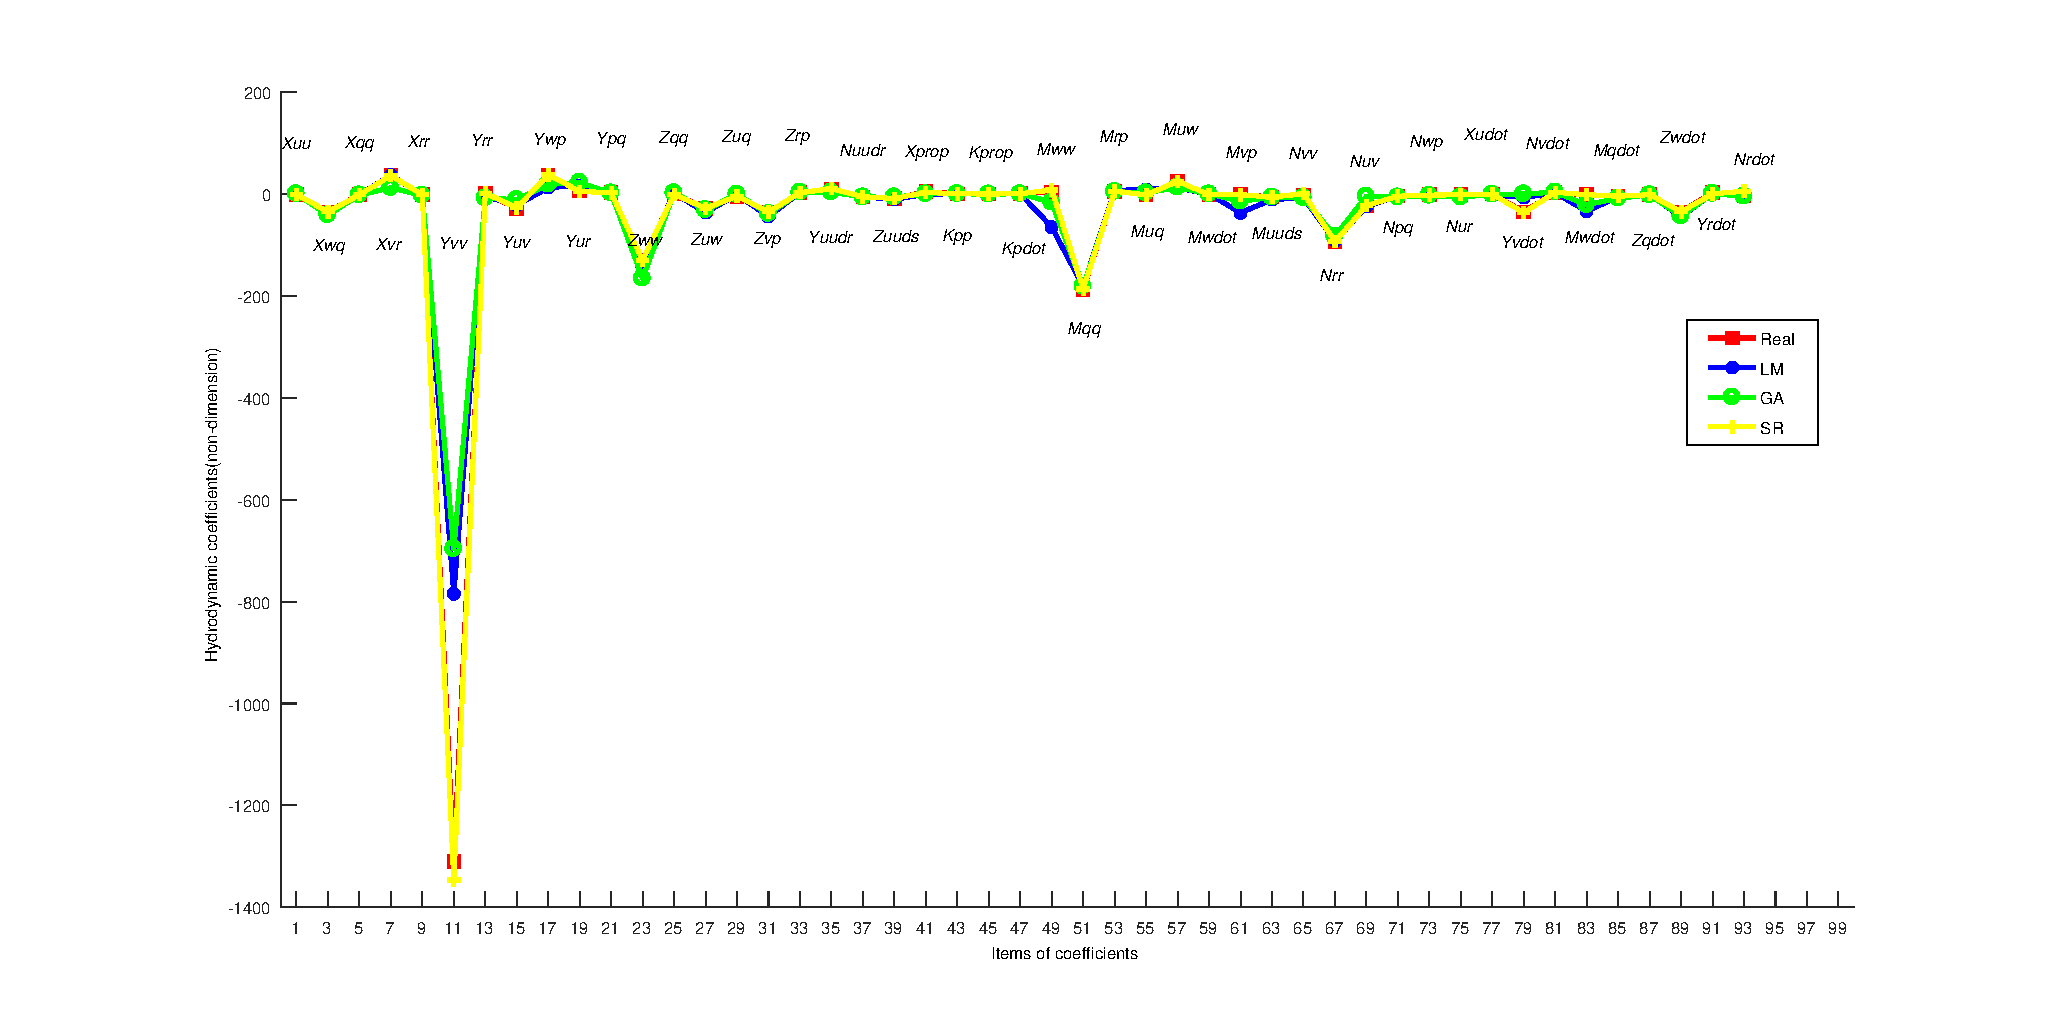
\includegraphics[width=1\textwidth]{figure/chap3/four_full.eps}
\label{fig:chap3:F4}
\bicaption[fig:chap3:F4]{使用LM、GA、SR方法进行AUV水动力参数辨识性能总体对比}{使用LM、GA、SR方法进行AUV水动力参数辨识性能对比} {Fig.}{AUV hydrodynamic coefficients comparisons between LM, GA, SR and Real Model}
\end{figure}

\begin{figure}[!htp]
\centering
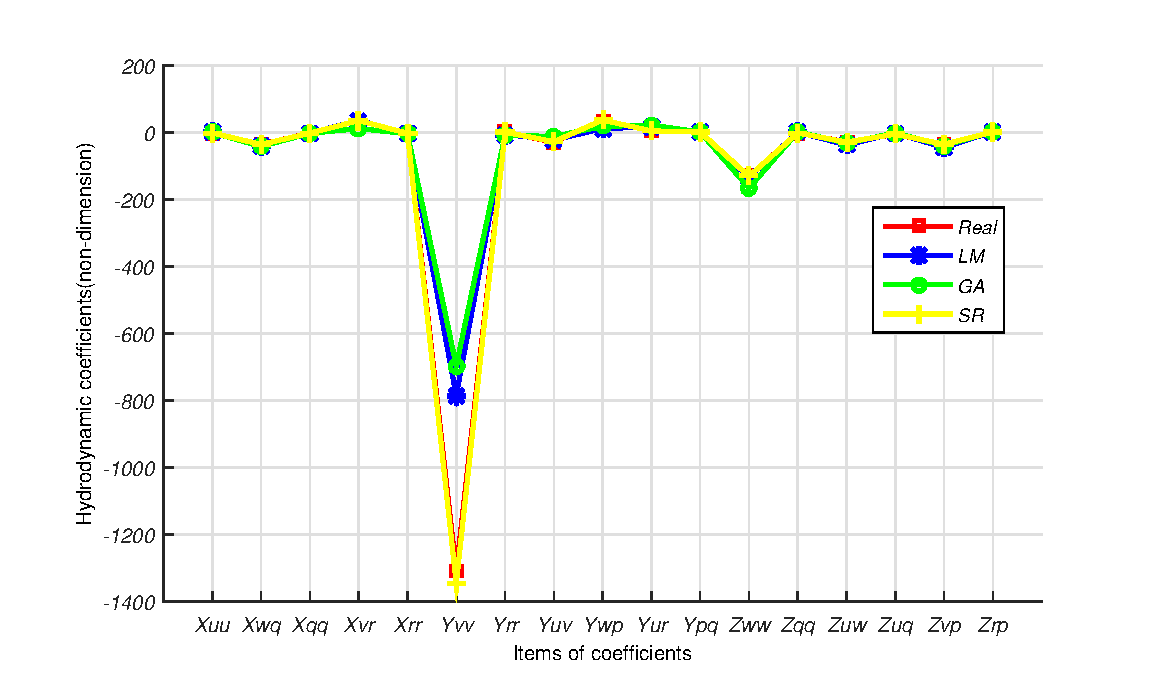
\includegraphics[width=14cm]{figure/chap3/four_1_17.eps}
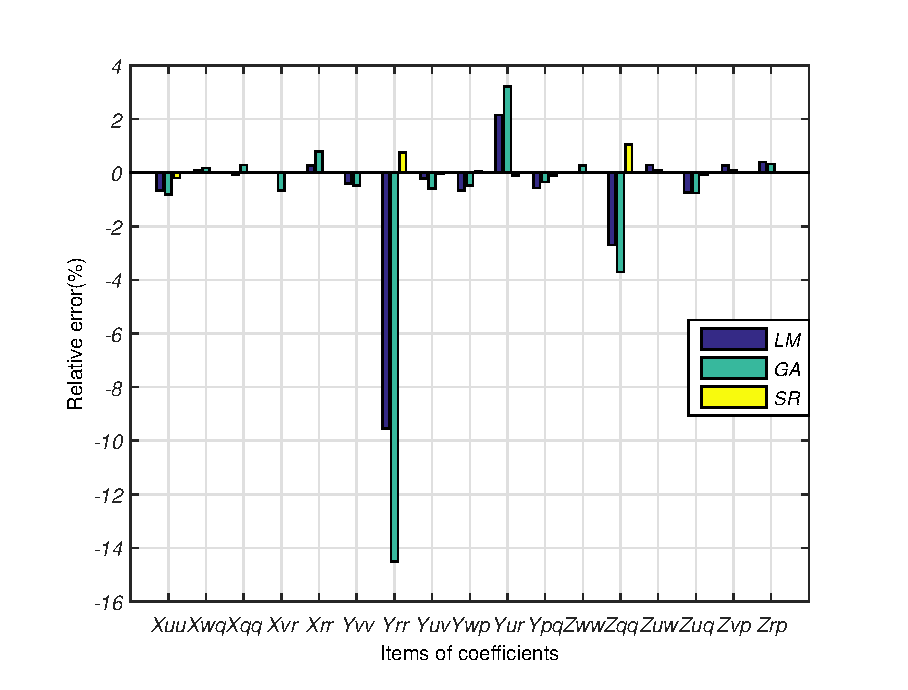
\includegraphics[width=14cm]{figure/chap3/relative_error_1_17.eps}
\label{fig:chap3:F5}
\bicaption[fig:chap3:F5]{使用LM、GA、SR方法进行AUV水动力参数辨识性能对比(1-17参数)}{使用LM、GA、SR方法进行AUV水动力参数辨识性能对比(1-17参数)} {Fig.}{AUV hydrodynamic coefficients comparisons between LM, GA, SR and Real Model(1-17)}
\end{figure}

\begin{figure}[!htp]
\centering
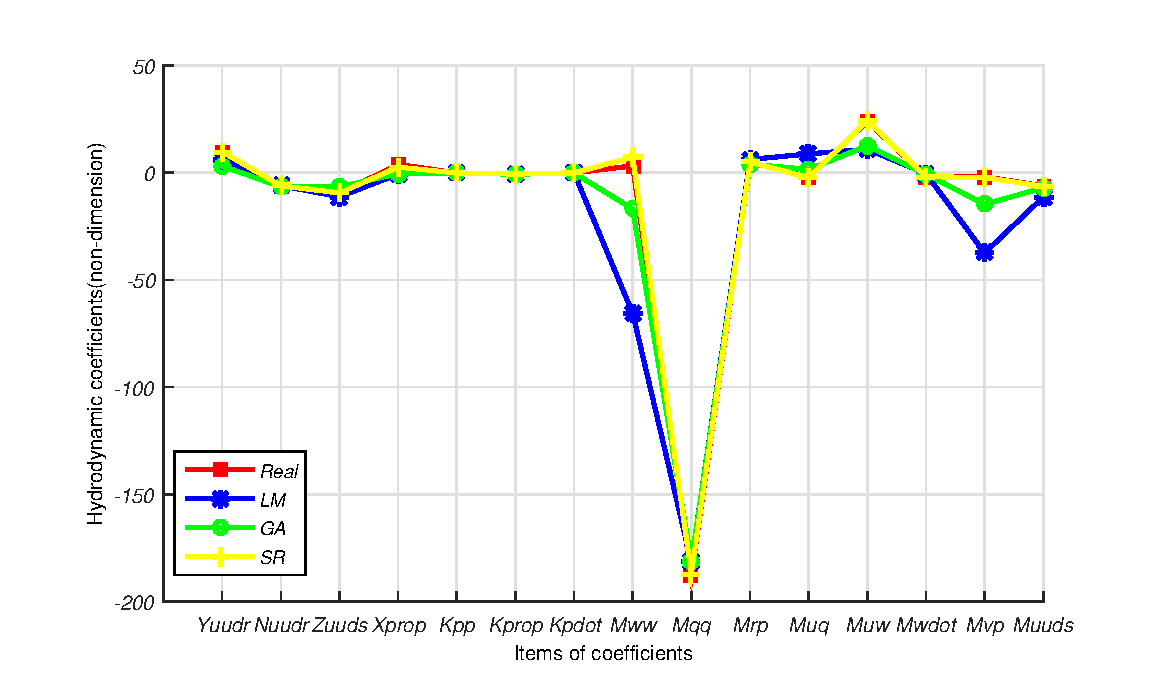
\includegraphics[width=14cm]{figure/chap3/four_18_32.eps}
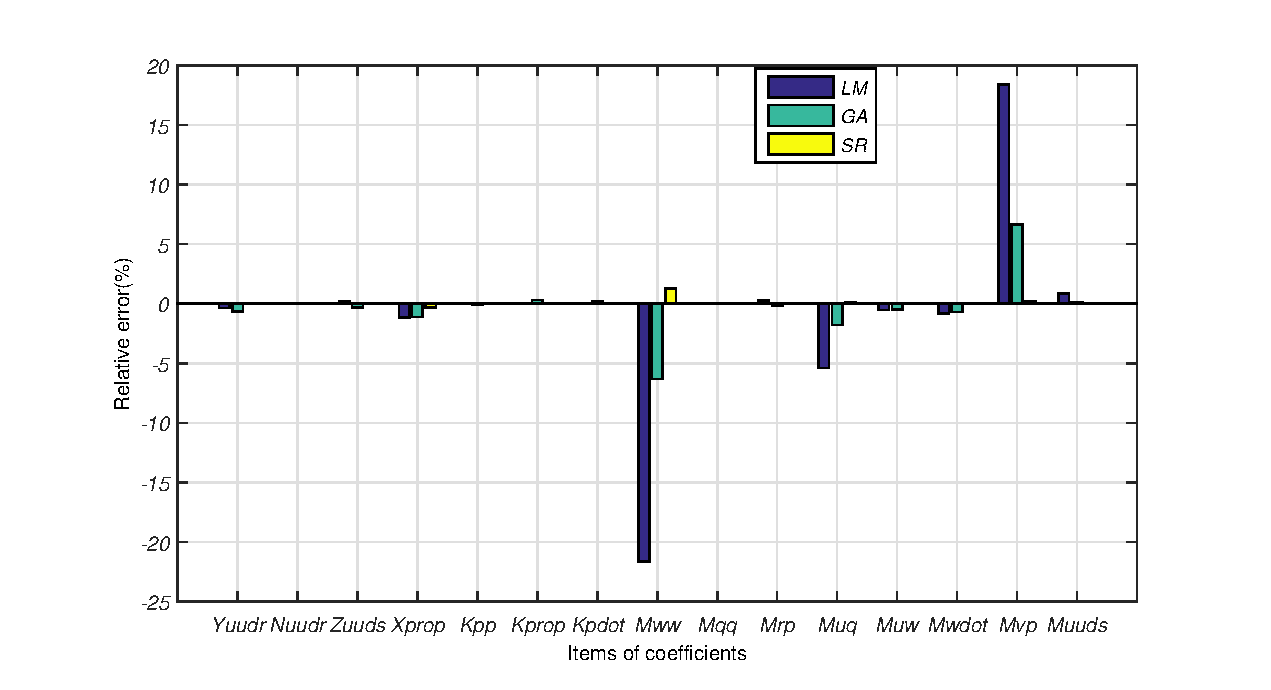
\includegraphics[width=14cm]{figure/chap3/relative_error_18_32_.eps}
\label{fig:chap3:F6}
\bicaption[fig:chap3:F6]{使用LM、GA、SR方法进行AUV水动力参数辨识性能对比(18-32参数)}{使用LM、GA、SR方法进行AUV水动力参数辨识性能对比(18-32参数)} {Fig.}{AUV hydrodynamic coefficients comparisons between LM, GA, SR and Real Model(18-32)}
\end{figure}

\begin{figure}[!htp]
\centering
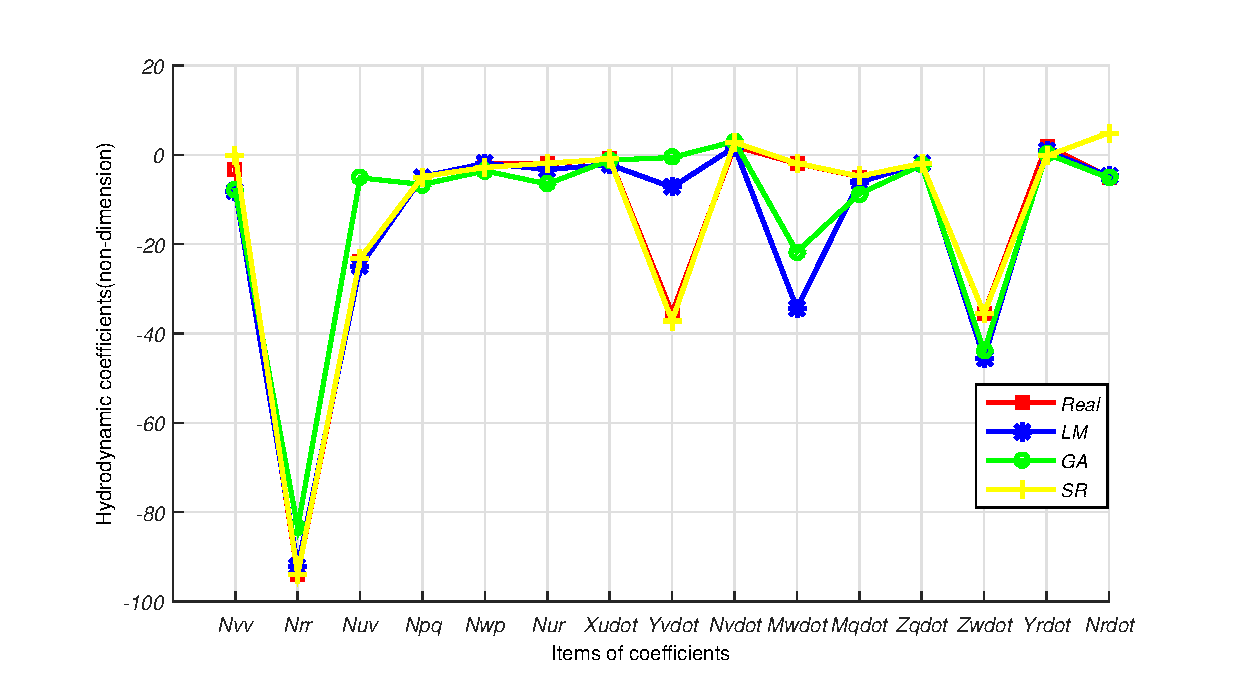
\includegraphics[width=14cm]{figure/chap3/four_33_47.eps}
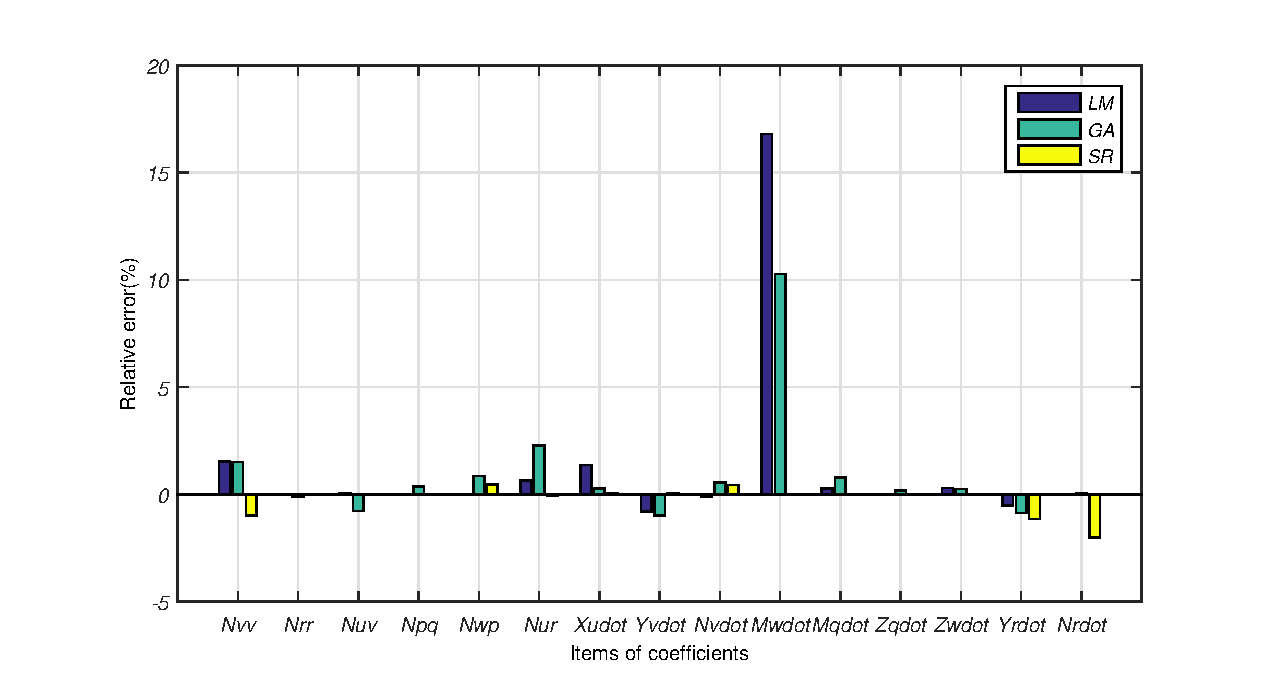
\includegraphics[width=14cm]{figure/chap3/relative_error_33_47.eps}
\label{fig:chap3:F7}
\bicaption[fig:chap3:F7]{使用LM、GA、SR方法进行AUV水动力参数辨识性能对比(33-47参数)}{使用LM、GA、SR方法进行AUV水动力参数辨识性能对比(33-47参数)} {Fig.}{AUV hydrodynamic coefficients comparisons between LM, GA, SR and Real Model(33-47)}
\end{figure}

遗传算法也可以识别水下航行器的参数,但搜索范围应适当地设置。 为了获得参数估计的良好结果, 最大遗传代数, 种群规模,交叉和变异概率分别为500, 80, 0.7, 0.02。

C. 参数辨识结果对比

图\ref{fig:chap3:F4} 将LM,GA,SR的辨识结果与实际模型系数进行比较。辨识的流体动力学系数基本上与模型的实际参数吻合良好;然而,对于一些系数,使用GA和LM算法估计的参数数值与实际参数数值相比,差异较大。 GA在一定程度上改善了水动力参数(如$Mww$,$Muq$,$Mvp$,$Mwdot$,$Zwdot$)的估计效果,但根据用于评估GA的参数识别的总体性能表\ref{tab:chap3:table1}中的MSE和STD的计算结果与使用LM方法相比,两者没有太大差异。此外,GA的搜索范围由LM的计算结果确定的,GA估计的过程非常耗时,而LM和SR更高效、计算更快,因为他们从开始估计的 100 秒内误差就收敛到一个很小的范围内。只不过, LM方法,由于会存在落入局部最优解的可能,容易在一次性搜索的过程中失败。对于符号回归方法,所有系数都是在选取数据集的50%和50%的情况下进行的模型训练和测试,这可以保持提出的方法的有效性。通过设置AUV的六个目标方程来确定所有参数。在图\ref{fig:chap3:F4}中的 $Yvv$ (也可见图\ref{fig:chap3:F5})和 $Yvdot$ (也可见图\ref{fig:chap3:F7})中显示出良好的一致性,其中 $dot$表示每个速度的导数。SR估计的模型参数的相对误差远小于由GA和LM识别的模型参数的相对误差,这说明了SR方法具有良好的参数识别能力。

\begin{table}[!t]
  \centering
  \label{tab:chap3:table1}%
  \bicaption[tab:chap3:table1]{LM, GA, SR方法的MSE和STD结果对比}{LM, GA, SR方法的MSE和STD结果对比}{Table}{Comparisons of MSE and STD between LM, GA and SR}
  \begin{tabular}{cccc}
  \toprule
        & MSE         & STD     & Processing time  \\
  \midrule
    LM  & 6.0645e+03  & 78.3369 & 33min            \\
    GA  & 8.1315e+03  & 90.4354 & 2h               \\
    SR  & 31.1485     & 5.6254  & 16min8s          \\
  \bottomrule
  \end{tabular}%
\end{table}%


为了进一步研究噪声对搜索过程的影响,根据收敛和参数辨识的效果,选择使用SR和LM方法来识别不同信噪比SNR传感器采集的带噪声运动数据。

如表\ref{tab:chap3:table2}所示,MSE和STD是LM方法识别的模型系数和实际力系数比较的评价标准,而最大误差,MSE和MAE是SR方法的收敛性评价标准; 在实验中,随着SNR的值的增大,两种方法都实现了收敛过程速度的显着提高,这里设定的条件是LM和SR的搜索时间均为8分钟; 而由于传感器质量的差异,传感器的质量越差,通过将识别结果进行比较,发现LM方法辨识的结果的性能评估标准会变得数值较大。

\begin{table}[!t]
\centering
\label{tab:chap3:table2}
\bicaption[tab:chap3:table2]{不同SNR模型数据的辨识效果对比}{不同SNR模型数据的辨识效果对比}{Table}{Evaluation of identification results and measured performance along with SNR}
\begin{tabular}{ccccccc}
\toprule
                       & SNR   &       1   & 10       & 20       & 45       & No noise \\
\midrule
\multirow{2}{*}{LM}    & MSE   & 194235    & 115055   &53575     &21412     &17937      \\
                       & STD   & 438.0196  & 333.6798 &227.4539  &  145.9737  &  132.549  \\
\midrule
\multirow{3}{*}{SR}    & Maximum Error & 49.9913 &19.06  & 6.4719  &0.4098 & 0.0118      \\
                       & MSE           & 227.2457  &  38.49  & 3.7726 & 0.0127 & 1.39E-05 \\
                       & MAE           & 12.1192& 4.9485  &1.5513  &0.089  & 0.0027        \\
\bottomrule
\end{tabular}
\end{table}

此外,为了验证SR在处理非连续数据方面的优势,我们将具有SNR等于45的相同测量运动数据放在一起,并重复使用SR方法进行参数识别。 在100秒内,SR目标函数的MAE仍收敛于小于0.1的值,最后经过20min17sec后得到MAE = 0.00136003,MSE = 0.0000036257619的结果。 REMUS第一自由度纵荡运动的流体力学系数的搜索结果如表\ref{tab:chap3:table3}所示。此外,我们还从各种运动状态数据集中随机选择数据构成新的辨识数据集,然后获得了REMUS模型的参数,这说明SR方法不仅 具有良好的收敛性,也可以获得更加准确的参数识别结果。同样也说明使用非连续数据集进行水动力系数识别SR方法也表现出出色的性能。

\begin{table}
\centering
\label{tab:chap3:table3}
\bicaption[tab:chap3:table3]{非连续数据集的符号回归辨识}{非连续数据集的符号回归辨识}{Table}{Identification parameters using noncontinuous motion data with SR}
\begin{tabular}{cccc}
\toprule
             &Real coefficients & Steering angle is same & Random Selected data\\
\midrule
 $X_{uu}$    & -1.62 &-1.620937076   & -1.606133018 \\
 $X_{\dot u} $   &-0.93  &-0.951148025   & -0.644722161 \\
 $X_{wq}$    &-35.5  & -35.53024222  & -34.85176751  \\
 $X_{qq}$    &-1.93  &  1.939137984  &1.953199585   \\
 $X_{vr}$    &35.5   & 35.53904256   &34.83378219  \\
 $X_{rr}$    &-1.93  &  -1.935145734 &-1.925233784  \\
 $X_{prop}$    &3.86   & 3.861580558   &3.919602871  \\
\bottomrule
\end{tabular}
\end{table}

如表 \ref{tab:chap3:table4}所示,使用Eureqa软件进行了水下航行器功能结构形式的搜索测试,这有助于研究者为REMUS AUV 的纵荡自由度运动找到一些有用的新的表达形式的模型,并给出模型的外力的表达形式,这对于确定水下机器人的简化数学模型非常有帮助。

在图\ref{fig:chap3:F8}和表\ref{tab:chap3:table4}中,给出了不同于非线性模型的外部力的新的表达形式,这是使用结构搜索发现的模型的另一种简化表达。AUV的受到的实际力和简化模型的估计的力之间的预测值是一致的,并且具有稳定性,这表明了所提出的方法适合用于模型的结构搜索。

\begin{table}
\centering
\label{tab:chap3:table4}
\bicaption[tab:chap3:table4]{AUV模型的结构搜索}{AUV模型的结构搜索}{Table}{Structure searching for AUV model}
\begin{tabular}{cc}
\toprule
Target expression & $\begin{array}{l}
 \dot u = {f_1}\left( {u,v,w,p,q,r,\dot v,\dot w,\dot p,\dot q,\dot r,delt{a_s},{\mathop{\rm de}\nolimits} lt{a_r}} \right) \\
  + {f_2}\sin \left( {theta} \right) \\
 \end{array}$  \\
\midrule
Function sets  & Constant,+,- ,*,/,abs() \\
\tabincell{c}{Search function \\ modal for surge} & $\begin{array}{l}
 \dot u = 2.45vr + 0.0342\sin (theata) - 2.2255wq \\
  - 0.1560q\^3 - 0.3914 \\
 \end{array}$ \\
\tabincell{c}{Search for external forces \\in the freedom of sway} & $\sum {FY}  = 3.3217 + 15.6577ur - 753.4552v\left| v \right|$ \\
\bottomrule
\end{tabular}
\end{table}

\begin{figure}[!htp]
\centering
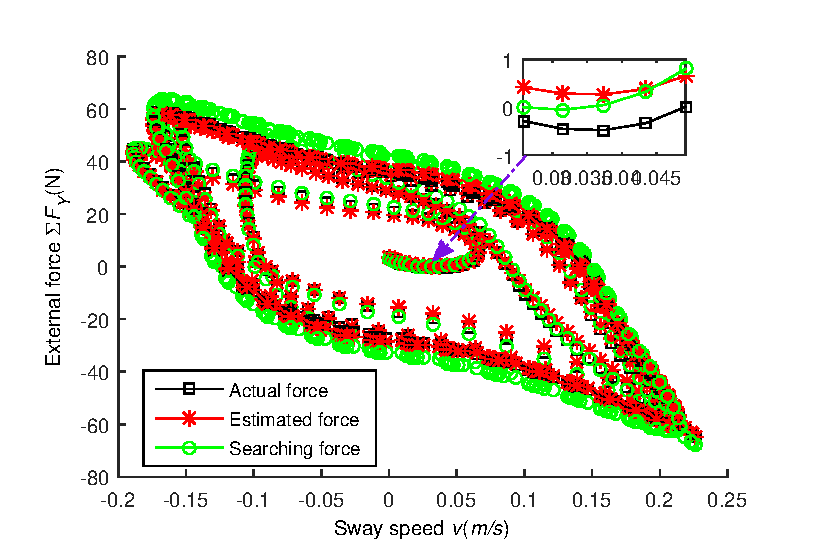
\includegraphics[width=14cm]{figure/chap3/search_compare.eps}
\includegraphics[width=14cm]{figure/chap3/time-force_compare.eps}
\label{fig:chap3:F8}
\bicaption[fig:chap3:F8]{实际、估计与搜索的外部力对比}{实际、估计与搜索的外部力对比} {Fig.}{comparisons of AUV external force on sway freedom between Actual, Estimated and Searching forces}
\end{figure}

在本节中,已经使用多种方法辨识和搜索了AUV模型的参数和结构。将模型的实际阻尼系数的值用作真值,然后与估计值进行比较。 非线性模型的辨识效果是使用LM算法、遗传算法和基于遗传编程的符号回归三种方法进行估计,并得到了水动力学模型参数。此外,还讨论并确认了传感器模型的影响以及符号回归方法的优点。最后,使用符号回归方法搜索AUV的模型结构。 结果表明,符号回归可以比LM和GA方法更准确地确定非线性模型的模型参数,并且还可以搜索数据集以获得AUV模型的表达形式,可以发现新表达形式。 因此,符号回归更适用于AUV系统建模。


\section{水流环境识别 }

水下航行器工作的水下环境对于其能够正常工作和作业至关重要,尤其是深海环境中存在的水流环境,本节主要研究
AUV型的水下机器人在水流环境中的感知问题\cite{verschure2003environmentally,fossen1994guidance}。首先介绍从鱼类生物学启发感知中找寻到研究灵感,发现鱼体侧线因受到水流变化而产生的神经冲动,不断地刺激鱼类的前端神经和大脑,使得鱼类可以感知水流的方向,利用水中存在能量完成巡游。其次,神经脉冲信号处理的过程类似于一个从大量数据学习水流模式的过程\cite{abdulsadda2013underwater,abdulsadda2012artificial,yang2010artificial,ren2012model}。典型的机器学习可以用来训练用于区分水流模式的模型\cite{liu2012support}。不过,应当考虑大规模传感器数据的信息稀疏特性,对其进行预处理\cite{chen2000new}。压缩感知可以用来处理大量的传感器数据,而能代表数据最大特性的一般就是其带有分类特性的特征向量。线性判别分析是一类可以压缩高维数据并带有分类特性的处理方法,因此本章将采用线性判别分析对数据进行预处理\cite{chen2000new,martis2013ecg}。最后,为了选择出保持分类的高正确率的分类器,选择使用了支持向量机,并对比多种内核的特性,训练出水流模型的方向分类器,并进行测试。

\subsection{鱼类侧线感知系统 }

鱼类拥有一个能够对周围水下环境感知运动的微机械感应侧线系统。它分布于鱼皮肤的两侧,主要由神经丘和侧线管组成(图\ref{fig:chap3:F9}与\ref{fig:chap3:F10})。神经丘体位于鱼体表皮上并向外凸起,使得它能够侵润到外部流体中,侧线管组成了侧线系统的大部分,每隔一个微小距离就通过侧线孔与外界流场相连。外部流体通过侧线管中液体的流动可以将流场中水内外声波,压力,水流速度改变信息传递给神经丘,神经丘的感觉神经细胞受到刺激通过神经纤维,经侧线神经传递到鱼的大脑。

    \begin{figure}[!htp]
    \centering
        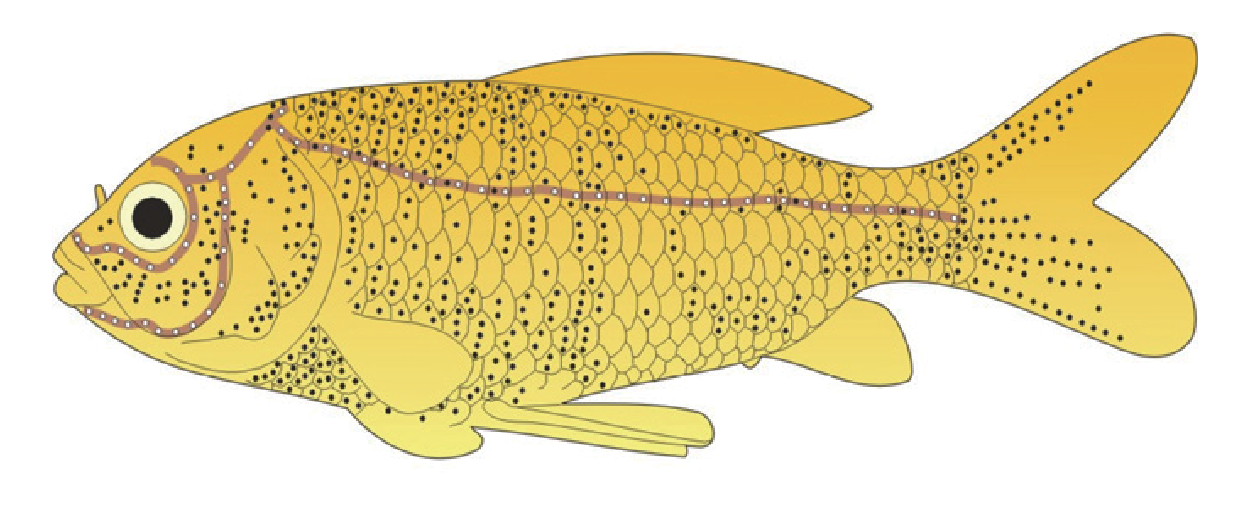
\includegraphics[width=11cm]{figure/chap3/fig1.jpg}
        \label{fig:chap3:F9}
        \bicaption[fig:chap3:F9]{鱼体侧线位置示意(棕色线)}{鱼体侧线位置示意(棕色线)} {Fig.}{Location of fish lateral line system(Brown)\cite{abdulsadda2012artificial} }
    \end{figure}

    \begin{figure}[!htp]
    \centering
        \includegraphics[width=14cm]{figure/chap3/fig2.jpg}
        \label{fig:chap3:F10}
        \bicaption[fig:chap3:F10]{鱼侧线局部放大示意图}{鱼侧线局部放大示意图:$1$ 水 $2$ 神经丘 $3$ 侧线管 $4$ 侧线孔 $5$ 表皮 $6$ 真皮} {Fig.}{enlarged partial schematic of fish lateral line:$1$ Water $2$  Neuromast  $3$ Lateral line tubes $4$ Lateral line pores $5$ Epidermis 6 Dermis  }
    \end{figure}

\subsection{基于支持向量机的水下机器人水流环境辨识  }

\subsubsection{流体控制方程 }
建立的模型是为了求解AUV本体周围的水流问题,用以提取二维面内的侧线节点压力数据。该模型是基于雷诺平均纳维-斯托克斯(Reynolds Averaged Navier–Stokes,RANS)方程。 对于湍流情况,速度场和水流场能够划分为两个部分:均值速度$<u_{i}>$ 与压力 $<p_{i}>$ , 湍流速度 $u_{i}^{'}$ 与压力 $p_{i}^{'}$。 这样 $u_{i} =  < u_{i} >  + u_{i}^{'}$ ,$p_{i} =< p_{i} >+p_{i}^{'}$,其中二维流分析 $i=1, 2$。如果流体假设是不可以压缩的,那么平均水流场主要是有RANS方程的情况:
\begin{equation}
\label{eq:chap3:14}
\frac{{\partial {U_j}}}{{\partial {x_j}}} = 0
\end{equation}

\begin{equation}
\label{eq:chap3:15}
\frac{{\partial {U_i}}}{{\partial t}} + \frac{\partial }{{\partial {x_j}}}\left( {{U_i}{U_j}} \right) = \frac{1}{\rho }\frac{{\partial P}}{{\partial {x_j}}}\left( {{\Gamma _{ij}} - \rho \bar u_i^{'}\bar u_j^{'}} \right)
\end{equation}
其中,$\rho$是流体密度,雷诺应力张量为\\

\begin{equation}
\label{eq:chap3:16}
 - \rho {{\bar u_i}^{'}}{{\bar u_j}^{'}} = \left[ {\begin{array}{*{20}{c}}
   { - \rho \bar u{{_1^{'}}^2}} & { - \rho {\bar u_1^{'}}{\bar u_2^{'}}}  \\
   { - \rho {\bar u_2^{'}}{\bar u_1^{'}}} & { - \rho \bar u{{_2^{'}}^2}}  \\
\end{array}} \right]
\end{equation}

$k-\varepsilon$ 模型是一种外部空气和流体动力学应用最广泛的湍流模型\cite{lamb1932hydrodynamics}。 因此文中选用其作为模拟航行器周表压力的湍流模型。

$k$函数\\

\begin{equation}
\label{eq:chap3:17}
\frac{{\partial \rho k}}{{\partial t}} + \nabla \left( {\rho \bar Uk} \right) = \nabla \left[ {\left( {\mu  + \frac{{{\mu _t}}}{{{\sigma _k}}}} \right)\nabla k} \right] + {P_k} - \rho \varepsilon
\end{equation}

$\varepsilon$函数\\

\begin{equation}
\label{eq:chap3:18}
\frac{{\partial \rho \varepsilon }}{{\partial t}} + \nabla \left( {\rho \bar U\varepsilon } \right) = \nabla \left[ {\left( {\mu  + \frac{{{\mu _t}}}{{{\sigma _k}}}} \right)\nabla \varepsilon } \right] + \frac{\varepsilon }{k}\left( {{C_{\varepsilon 1}}{P_k} - {C_{\varepsilon 2}}\rho \varepsilon } \right)\end{equation}

其中,\[{P_k} = {\mu _t}\nabla \bar U \left( {\nabla \bar U + \nabla {{\bar U}^T}} \right) - \frac{2}{3}\nabla {\bar U} \left[ \left( {3{\mu _t}\nabla } \bar U   + \rho k   \right)\right] \]

\[{\mu _t} = {C_\mu }\rho \frac{{{k^2}}}{\varepsilon }\]

文节研究的对象是一个鱼雷型AUV,模仿REMUS AUV 设计而成,它能够工作在水深100m区域并进行多项任务。整个模型是长圆柱型并有四个舵在尾部,其中有两个水平舵,两个垂直舵。关于体坐标系的Oxy 面和Oxz面对
称,因此AUV 运行分析的流体域简化为二维平面
流体域。整个计算模型是使用ICEM软件建立的1:1的网格模型。网格主要是三角型网格,网格节点数为18253。网格划分可以见图\ref{fig:chap3:F11}。流体域是个圆形水域,直径为15m,左侧为来流入口,右侧围出口,内部为AUV外边界,内边界根据AUV水下运动的特性为O型网格。

边界层设置:边界层的设置在ICEM和Fluent中完成,包括(1)流体域左半圆边界,流体域右半圆边界,因为来流方向是 $0, 45, 90, 135, 180, 225, 270,315$八个主要方向进行计算,入口出口的设置根据来流方向进行调整并设置不同的来流速度大小($0-3 m/s$);(2)内部边界是AUV的侧线提取数据边界,设为wall, 流体域为FLUID。 因为海中的深水水流主要是稳定的, 因此本次只进行稳定流场的计算。其中计算结果如图\ref{fig:chap3:F12}所示。

    \begin{figure}[!htp]
    \centering
        \includegraphics[width=10cm]{figure/chap3/fig4.jpg}
        \label{fig:chap3:F11}
        \bicaption[fig:chap3:F11]{流体网格模型}{流体网格模型} {Fig.}{Fluid mesh }
    \end{figure}

    \begin{figure}[!htp]
    \centering
        \includegraphics[width=13cm]{figure/chap3/fig5.jpg}
        \label{fig:chap3:F12}
        \bicaption[fig:chap3:F12]{45度水流计算流速图}{45度水流计算流速图} {Fig.}{Velocity profile for vehicle with 45 degree inflow }
    \end{figure}

\subsubsection{ 水流识别方法 }

水流的识别主要需要确定两个基本要素,即水流的方向和流速的大小。而建立水流预测模型要能够对这两点进行正确地估计。由于提取的压力数据节点较多,使用分类器直接训练,计算成本较高。而传感器数据的信息是稀疏分布的,有重要的,有不重要的。为了提取出来重要的数据特征信息,线性判别分析方法被用来处理压力传感器数据,并得到了很多代表流向特征的数据信息。将获得的特征信息输入到支持向量机建立的水流方向分类器里面,对分类器进行训练。在确定了水流的流向后,仍然有一个重要的要素需要注意,那就是水流的流速大小。要辨别流速大小并不容易,尤其是当水流的速度值较小的时候,因此使用拟合法来建立水流流速的预测方程,输入到方程里的是压力极值,输出是流速。如此就可以完成对水流的流速方向和大小的模式预测。并且,预测的处理也参考了鱼的层级处理结构\cite{yang2010artificial}。

A. {线性判别分析}

线性判别分析({Linear Discriminant Analysis})是一种监督式的机器学习方法,这种方法不是使用概率知识来训练和预测数据的模式的,因此线性判别分析并不需要关于数据的已知的先验和后验概率值。线性判别分析的主要思想是将输入的高维度的数据投影到一个较低的维度空间内。在这个空间中,数据的点将被划分为一个个的簇,并且这些簇之间保持一定的距离。这里提到簇就是所说的类的低维度空间的表示。线性判别分析采用的投影处理,可以让高维度的压力数据降低维度,并保持较好的分类特性,这是该方法的优点。下面将给出线性判别分析的主要理论。

线性判别分析从其名字就可以知道该方法属于线性分类器。这种分类器具有 $k$线性函数,而这些函数都是为了所需要划分的$K$类问题而定义。协方差矩阵被定义如下\cite{martis2013ecg,chen2000new}:

\begin{equation}
{S_W} = \sum\limits_{k = 1}^K {{S_{_k}}}
\label{eq:chap3:19}
\end{equation}
其中,
\begin{equation*}
\begin{aligned}
{S_k} &= \sum\limits_{n \in {C_k}} {\left( {{x_n} - {m_k}} \right){{\left( {{x_n} - {m_k}} \right)}^T}}\\
{m_k} &= \frac{1}{{{N_k}}}\sum\limits_{n \in {C_k}} {{x_n}}
\end{aligned}
\end{equation*}
式中$N_k$ 是 $C_k$ 的模式数目,$x_n$ 是第 $n$ 种模式的观测向量。$K$是数据样本中的整体分类数,该数定义与所采集数据的水流方向有关,本文中为8。

\begin{equation}
{S_B} = \sum\limits_{k = 1}^K {{N_k}\left( {{m_k} - m} \right){{\left( {{m_k} - m} \right)}^T}}
\label{eq:chap3:20}
\end{equation}
式中,
\begin{equation*}
m = \frac{1}{N}\sum\limits_{n = 1}^N {{x_n}}  = \frac{1}{N}\sum\limits_{k = 1}^K {{N_k}{m_k}}
%\label{equation:eq5}
\end{equation*}
$m$是所有数据的平均值。

所有样本的协方差矩阵给出如下:
 \begin{equation}
{S_T} = {S_W} + {S_B}
\label{eq:chap3:21}
\end{equation}

投影矩阵的方程给出如下:
\begin{equation}
W = {\arg _W}\max \left\{ {{{\left( {W{S_W}{W^T}} \right)}^{ - 1}}\left( {W{S_W}{W^T}} \right)} \right\}
\label{eq:chap3:22}
\end{equation}

线性判别分析的系数是从投影矩阵中获得的,给出的形式如下:

\begin{equation}
y = {W^T}x
\label{eq:chap3:23}
\end{equation}
式中,$y$是线性判别分析的系数,$x$ 是给定模式下的次级区域的 $DWT$ 系数。

当满足所有条件时:如果 $j$ 无论取任何值不等式$y_k>y_j$ 都成立,那么 $x$ 就属于第 $k$ 类。根据上面的方程,就可以分别求出每一类的评估数值。根据这些评估数值,就可以对样本进行分类和数据降低维度。

B. {支持向量机 }

前面的水流流体仿真中提出的压力数据是维度很高的,如果使用分类器进行直接处理,会加大计算的成本。而基于面向载体实验和应用的目的,需要将压力数据进行处理到较低的维度内。本部分介绍的分类器所输入的数据是基于前文使用线性判别分析方法预处理过的数据。从这些数据中获得的特征向量维度低,可以反映航行器体表的压力变化情况。支持向量机(Support Vector Machine)本身属于一种二分类方法,而水流的流向确是多种多样的。要建立流向的分类器,就需要将水流方向模式的判别问题转为多个循环的标准问题来解决。支持向量机可以对数据进行泛化处理,即使数据的样本有限,也能很好判别数据的模式。因此提出的分类器选择使用支持向量机来进行整体的模式识别,下面给出支持向量机的相关理论。具体描述如下:

\begin{equation}
V = \left\{ {\left( {{x_{1,}}{y_1}} \right),...,\left( {{x_i},{y_i}} \right)} \right\}
\label{eq:chap3:24}
\end{equation}
式中,$i=1,2,\ldots$,${x_i} \in {R^n}$,${y_i} \in \left\{ { \pm 1} \right\}$。

超平面为${\omega ^T}X + b = 0$,并且 $x_i$ 是需要处理的特征向量,$y_i$ 是需要识别的模式,$\omega$ 是标准向量,$b$ 是偏差项。

支持向量机分类器的主要目的是找出一个最优的超平面,这个平面可以几乎没有错误地区分模式。经过这样的处理,最近向量到超平面间的距离就是最大的。对参数化过程进行限制,就可以得到特定的最优超平面:

\begin{equation}
\min \frac{1}{2}{\left\| {\left. \omega  \right\|} \right.^2}
\label{eq:chap3:25}
\end{equation}
\begin{equation*}
\begin{array}{*{20}{c}}
   {s.t.} & {{y_i}\left( {{\omega ^T}{x_i} + b} \right) \ge 1,\begin{array}{*{20}{c}}
   {} & {i = 1,2,...,m}  \\
\end{array}}  \\
\end{array}
\end{equation*}
可以发现,当 $y_i=-1$ 时,$\bm{\omega}^T\bm{X}+\bm{b} \leq 0$,反之,则当 $y_i=1$ 时,$\bm{\omega}^T\bm{X}+\bm{b} > 0$。

将拉格朗日鞍点理论与经典拉格朗日对偶问题结合在一起,并求解方程\ref{eq:chap3:25},就可以将求解问题转为二值问题:

\begin{equation}
\max \sum\limits_{i = 1}^m {{\alpha _i} - \frac{1}{2}\sum\limits_{i = 1}^m {\sum\limits_{j = 1}^m {{\alpha _i}\left( {{y_i}{y_j}{x_i}{x_j}} \right)} {\alpha _j}} }
\label{eq:chap3:26}
\end{equation}

\begin{equation*}
\begin{array}{*{20}{c}}
   {s.t.} & {\sum\limits_{i = 1}^m {{\alpha _i}{y_i} = 0,{\alpha _i} \ge 0} }  \\
\end{array}
\end{equation*}
式中,$\alpha$是拉格朗日算子,可以从方程\ref{eq:chap3:26}中获得。

根据上面公式,就可以得到最佳超平面的数学表达:
\begin{align}
  {\omega ^*} &= \sum\limits_{i = 1}^m {{\alpha _i}{y_i}{x_i}}
  \label{eq:chap3:27}\\
  {b^*} &=  - \frac{1}{2}{\omega ^*}^T\sum\limits_{i = 1}^m {\left( {{x_p} + {x_q}} \right)}
  \label{eq:chap3:28}
\end{align}
式中,$x_p$, $x_q$是每个模式的支持向量。

可以给出支持向量机的一个分类器:

\begin{equation}
\nu \left( x \right) = sign\left( {\sum\limits_{i = 1}^m {\left( {{\alpha _i}{y_i}{x_i}x + b} \right)} } \right)
\label{eq:chap3:29}
\end{equation}

支持向量机的方法是使用MATLAB实现的,为了选出最优的分类器,对支持向量机的各种内核函数,如线性核函数,二次核函数,多项式核函数,高斯径向基函数,多层感知核函数,都进行了测试与对比。分类器的对比结果将在下一部分给出。

\subsection{结果与分析 }

本部分采取四个步骤来训练和测试压力节点的所有数据,其中传感器数据在图\ref{fig:chap3:F13}, \ref{fig:chap3:F14}和\ref{fig:chap3:F15}中所示。 每个图中的曲线的特征在形状上是相似的,尽管速度和压力的大小值不同,但是这为进行水流预测提供了直接可分类证据。另外,获得的压力数据由于水流的流向不同,也会出现变化,可以参考图\ref{fig:chap3:F13},\ref{fig:chap3:F14} 和 \ref{fig:chap3:F15}。为了分析水下机器人运动对于分类的影响,本部分提出了三个权重标准用来衡量分类器的性能。根据每个类的内核测试结果,可以选出最佳支持向量机分类器的最优内核。经过数据压缩的预处理,从表征水流的高维度压力数据提取出来最优的特征向量。水流的另一个要素速度是使用压力的极大极小值的数据而拟合出一个流速预测方程。为了验证所提出的分类方法的可行性,最后使用水流分类器对随机选取的未被使用过的压力数据进行水流的流向和流速大小的预测。

    \begin{figure}[!htp]
        \centering
        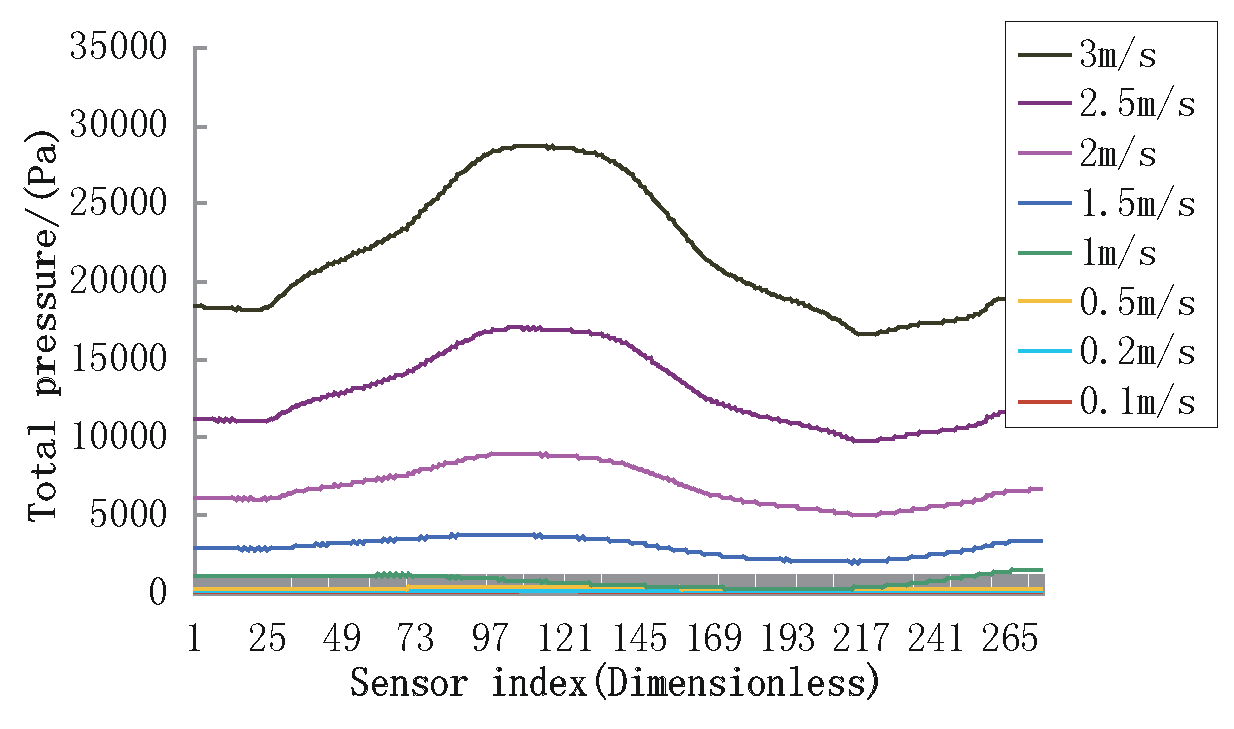
\includegraphics[width=11cm]{figure/chap3/fig6a_pressure_0.pdf}
        \label{fig:chap3:F13}
        \bicaption[fig:chap3:F13]{来流角为0度时的总压强对比}{来流角为0度时的总压强对比} {Fig.}{Comparison of total pressure with inflow angle is zero degree}
    \end{figure}
%    \hspace{0.5in}
%    \vspace{0.5in}
    \begin{figure}[!htp]
        \centering
        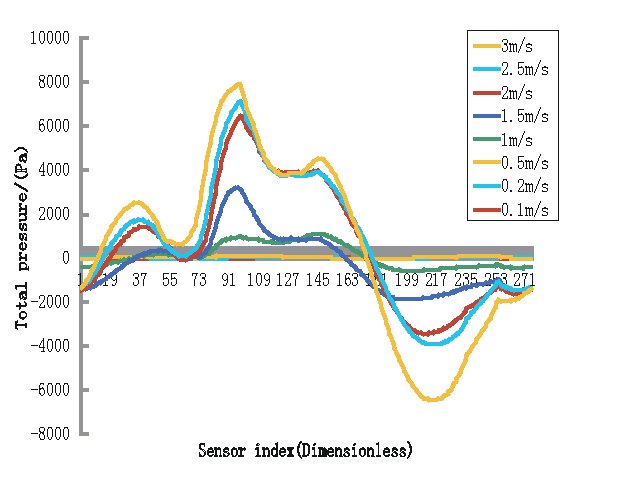
\includegraphics[width=11cm]{figure/chap3/fig6b_pressure_60.pdf}
        \label{fig:chap3:F14}
        \bicaption[fig:chap3:F14]{来流角为60度时的总压强对比}{来流角为60度时的总压强对比} {Fig.}{Comparison of total pressure with inflow angle is 60 degree}
        %\label{fig:pre60}
    \end{figure}

    \begin{figure}[!htp]
        \centering
        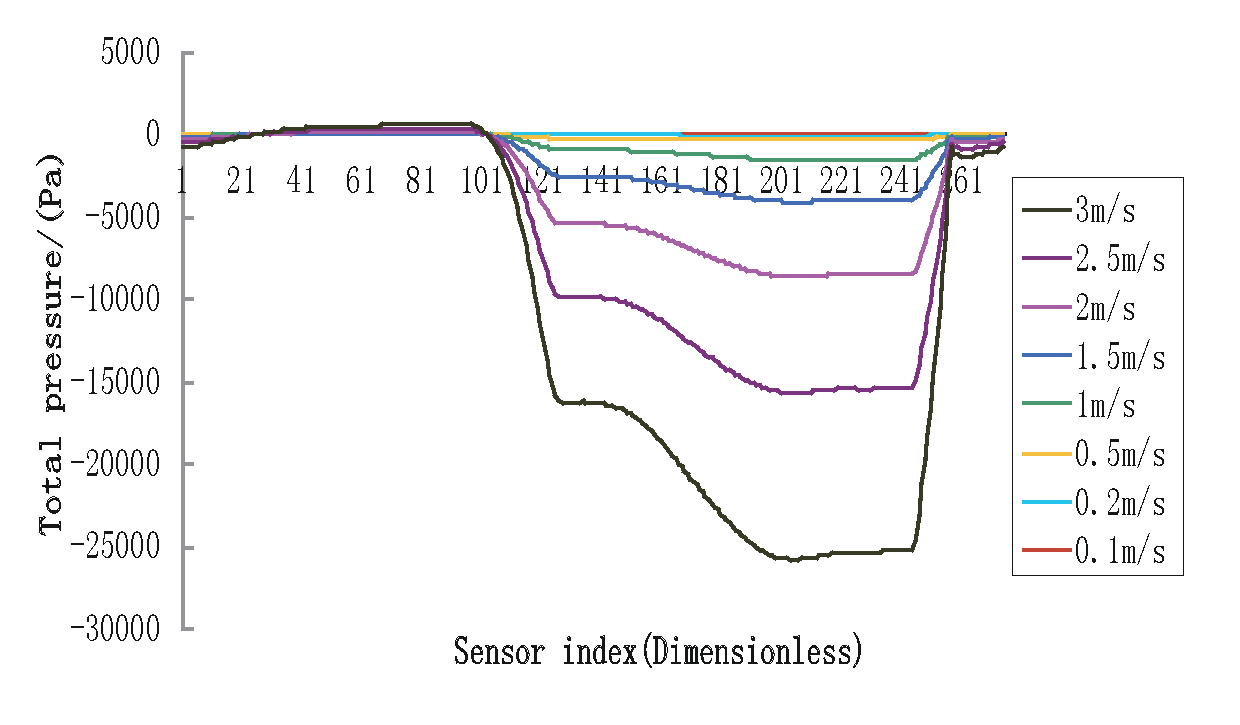
\includegraphics[width=11cm]{figure/chap3/fig6c_pressure_90.pdf}
        \label{fig:chap3:F15}
        \bicaption[fig:chap3:F15]{来流角为90度时的总压强对比}{来流角为90度时的总压强对比} {Fig.}{Comparison of total pressure with inflow angle is 90 degree}
        %\label{fig:pre90}
    \end{figure}
    % \bicaption[fig:fig6abc]{图}{不同来流的总压力比较:每个图中的图例表示流速的大小.} {Fig}{Comparison of total pressure of different flow: legends in each figure represent the magnitude of flow velocity. }


A. {测试运动评价权重}

本部分提出的三个权重标准被提出是用来评估航行器周围的瞬态冲击和能量分布情况。$W$ 是流速测试的一般权重,$Wv$ 是考虑流体冲击效应的速度评估权重,$Wvv$ 是用来反映能量分布情况的速度平方权重。三个权重的对比可以参考图\ref{fig:chap3:F16}。

\begin{figure}[!htp]
    \centering
        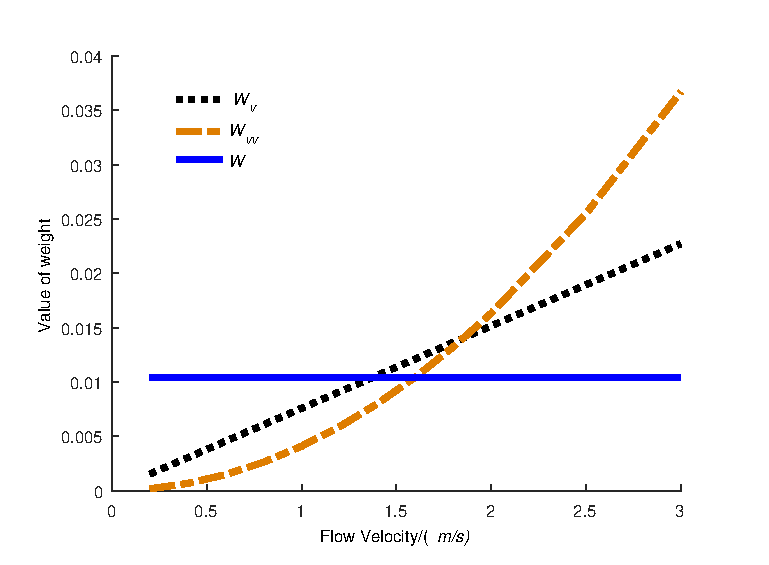
\includegraphics[width=10cm]{figure/chap3/fig7_weigiht_EnglishVersion.eps}
        \label{fig:chap3:F16}
        \bicaption[fig:chap3:F16]{不同的评价权重对比图}{不同的评价权重对比图} {Fig.}{Comparison of different weights}
\end{figure}

B. {选取最优支持向量机内核函数}

水流预测主要分为识别流向和估计流速大小,和人类感知风的情况相似,因此水流分类的工作侧重于流向的识别。 由于支持向量机有各种类型的内核函数,因此,使用不同的分类器测试了水流流向的辨识效果,并可以从表\ref{table:chap3:kenerls}中的测试结果选择出最佳的内核函数。

\begin{table}[!htp]
  \centering
  \label{table:chap3:kenerls}%
  \bicaption[table:chap3:kenerls]{不同内核的测试结果对比}{不同内核的测试结果对比} {Table}{Testing results for each kernel }
    \begin{tabular}{cccc}
    \toprule
    kernel type & $W$ & $W_v$    & $W_{vv}$ \\
    \midrule
    linear & 0.7708 & 0.9091 & 0.9436 \\
    Quadratic & 0.8438 & 0.9045 & 0.8847 \\
    Polynomial & 0.9271 & 0.9545 & 0.9462 \\
    RBF   & 0.7396 & 0.8333 & 0.8366 \\
    multilayer perception & 0.2185 & 0.247 & 0.2549 \\
    \bottomrule
    \end{tabular}%
\end{table}%

C. {特性提取 }

压力数据是从流体分析模型的航行器的体表上提出的,由于节点较多,提出的压力数据维度较高,因此为了便于后续处理,需要对数据进行预处理。基于压缩感知的思想,将数据压缩且不失去数据中的大部分信息是可行的。这里使用了线性判别分析对压力数据进行处理,预先标记一些数据,将数据投影到更低的维度,形成新的可以反映数据特征的特征向量。需要指出,特征向量的个数是由标记的数据的类的个数来定,这里的最大特征向量个数为7个。将获得的特征向量输入到分类器里面,并进行不同运动效应下的分类效果对比,如表\ref{table:chap3:sevenvector}。

% Table generated by Excel2LaTeX from sheet 'Sheet1'
\begin{table}[!htp]
  \centering
  \label{table:chap3:sevenvector}%
  \bicaption[table:chap3:sevenvector]{七特征向量的分类效果}{七特征向量的分类效果} {Fig.}{LDA compressed SVM classification for seven feature vectors }
    \begin{tabular*}{7cm}{cccc}
    \toprule
    Weight type & \textit{W} & \textit{Wv} & \textit{Wvv} \\
    \midrule
    Correct rate & 0.9375 & 0.9697 & 0.9625 \\
    \bottomrule
    \end{tabular*}%
\end{table}%

AUV 运行的水下环境是实时多变的,为了更及时获取水流的方向模式,文中对所有的2个特征矢量组合选择进行测试,测试效果见图\ref{fig:chap3:F17},不同的特征矢量组合获得的测试效果呈现不同的差异,不同的评价权重也会得到不同的特征矢量选择。

\begin{figure}[!htp]
    \centering
        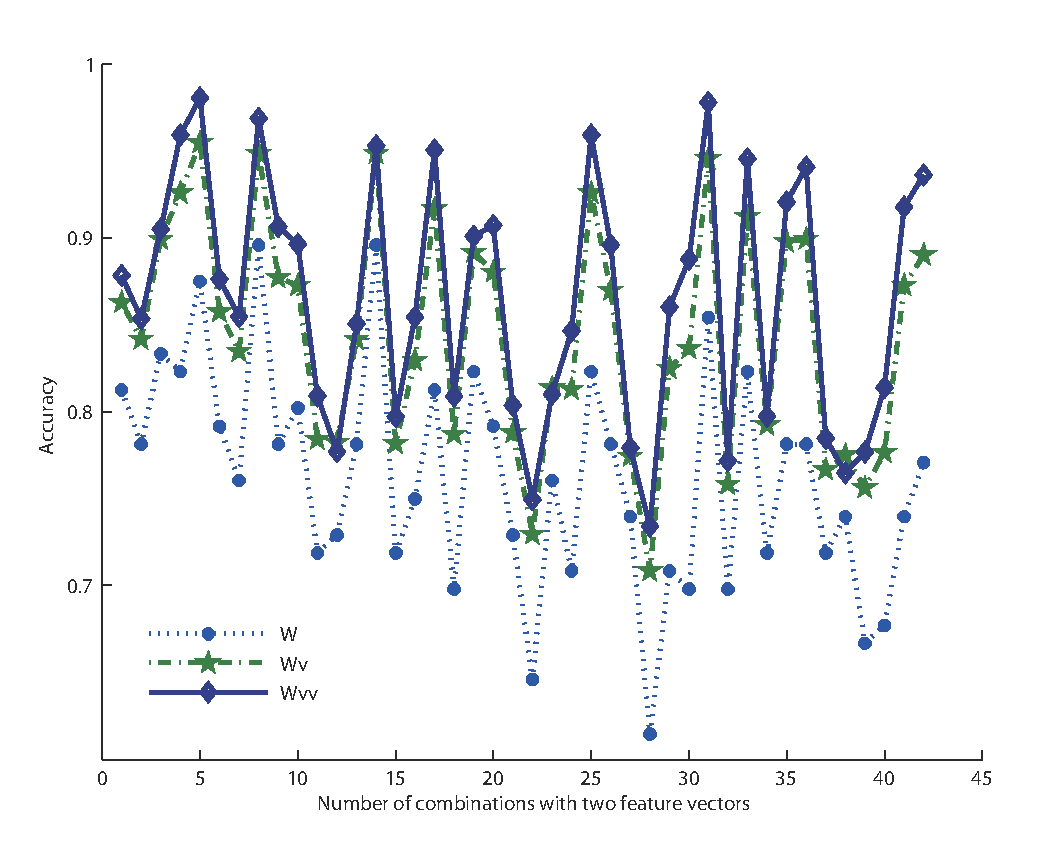
\includegraphics[width=14cm]{figure/chap3/fig8_Total_LDA_two_eigvalue_accurry_EnglishVersion1.pdf}
        \label{fig:chap3:F17}
        \bicaption[fig:chap3:F17]{两特征向量的组合分配测试效果}{两特征向量的组合分配测试效果} {Fig.}{Two feature vectors combined evaluation }
\end{figure}

D. {速度大小估计 }

不同的水流方向上水流速度的大小也是不同,由于不同水流的速度的作用,AUV 本体上受到的压力也是不同,图\ref{fig:chap3:F18} 为不同水流方向下不同流速的压力最大值最小值。为了在判定水流大小后,进而确定出水流的速率,文中使用速度与对应压力极值分别拟合各方向的水流值。拟合的测试270º 流向速度压力极值方程见图\ref{fig:chap3:F19}。

\begin{figure}[!htp]
    \centering
        %\noindent\makebox[\paperwidth][c]
        {
        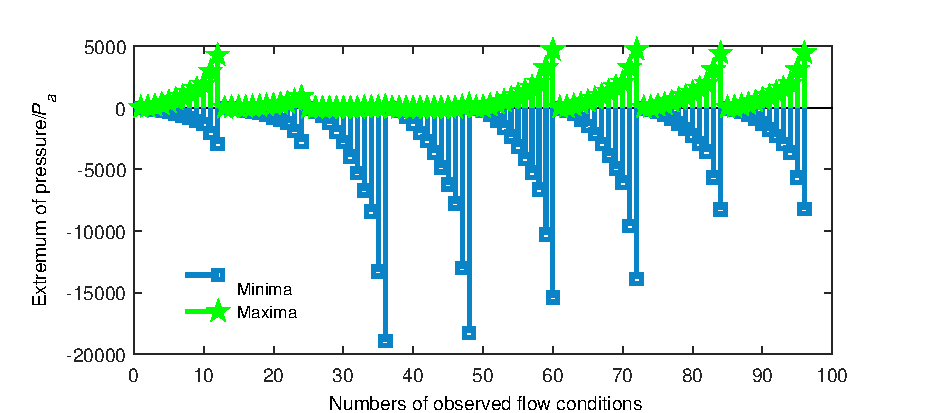
\includegraphics[width=14cm]{figure/chap3/fig9_press_value_maxmin_EnglishVersion1.eps}
        }
        \label{fig:chap3:F18}
        \bicaption[fig:chap3:F18]{压力数据极值}{压力数据极值} {Fig.}{Pressure extremes }
\end{figure}

\begin{figure}[!htp]
\centering
\subfigure[Maxima pressure $P_{max}/P_a$]{
\label{fig:chap3:F19a}
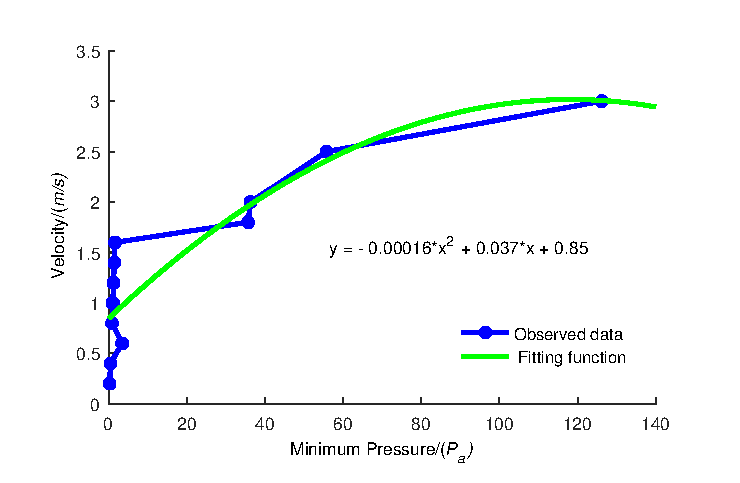
\includegraphics[width=10cm]{figure/chap3/fig10a_maximum.eps} }
\hspace{1in}
\subfigure[Minimum pressure $P_{max}/P_a$]{
\label{fig:chap3:F19b}
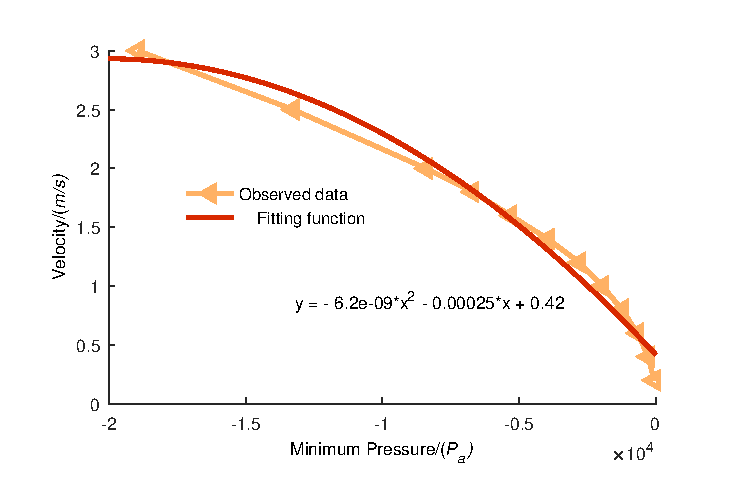
\includegraphics[width=10cm]{figure/chap3/fig10b_minimum.eps} }
\label{fig:chap3:F19}
\bicaption[fig:chap3:F19]{270度来流的流速预测方程}{270度来流的流速预测方程} {Fig.}{Fitting pressure equation of flow rate in 270-degree flow }
\end{figure}



\begin{table}[!htbp]
% %\tiny
%   %\onecolumn
  \centering
  \label{table:chap3:verification}
  \bicaption[table:chap3:verification]{水流预测结果}{水流预测结果}{Table}{Results comparison of flow forecasting }
  \begin{tabular}{ccccccc}
  \toprule
  \multirow{2}{*}{Flow direction estimation} & \multicolumn{4}{c}{Flow angle / $\left (degree\right )$} \\
                           &135    &270    &0      & 45    &90    &180 \\
  \midrule
  Actual flow rate/($m/s$) &1.8    &1.6    &1.8    &1      &1.6    &2.5 \\
      \\
  Test flow rate /($m/s$)  & 1.818 &1.2566 &1.1817 &0.888  &1.3226 &2.63 \\
  \bottomrule
  \end{tabular}%
\end{table}%

E. {分类器测试 }

为验证建立的水流方向模式识别模型与流速估计方法的有效性,以随意选取的且未被使用过的多个水流压力数据进行预测,获得如下测试效果(表\ref{table:chap3:verification})。

由表\ref{table:chap3:verification}可以验证,LDA-SVM 分类器能够有效地判断水流流向,并在一定范围内有效地计算出水流速度,这与生物感知空气场与流体场的结果相同。

F. {水下机器人运动学与水流预测模型的关系探讨   }

\begin{algorithm}[!htbp]
\centering
\caption{侧线估计偏航角的流程 \protect \\\quad \quad Framework of how to measure yaw angle based on lateral line}
\label{Algorithm:chap3:Framwork}
% \bicaption[Algorithm:chap3:Framwork]{侧向估计偏航角的框架流程}{侧向估计偏航角的框架流程}{Fig.}{Framework of how to measure yaw angle based on lateral line}
\begin{algorithmic}[1]
\REQUIRE
The pressure sensor node value around vehicle body is $P \left (t,i \right )$ at time $t$. The initial orientation angle of yaw motion, set $\psi_{t=0} =0$, and assuming the water environment is stable, so $V_{flow_{t}}$ is constant, and $R\left (\varphi,\theta,\psi  \right )\approx R\left ( \psi \right )$ in surface plane motion;\\

%The set of positive samples for current batch, $P_n$;
%The set of unlabelled samples for current batch, $U_n$;
%Ensemble of classifiers on former batches, $E_{n-1}$;
\ENSURE
The yaw angle of vehicle, $\psi_t$;
%Ensemble of classifiers on the current batch, $E_n$;
\FORALL{$t= j$ in $T$}
    \STATE forecast the velocity direction of flow: \\
    $ v_{direction} = f_{LDA-SVM}\left ( P \left (t,i \right ) \right )$;
    \STATE calculate the magnitude of flow velocity: \\
    $v_{magnitude} = w_1\ast g\left(min\left( P \left (t,i \right ) \right)\right)
    + w_2 \ast  h\left(max\left(    P \left (t,i \right )    \right)\right)   $, \\where $w_k =0.5$  is the component weight, $k = 1,2$;\\

    \STATE ${v_{flow_t}}$ is composed with $ v_{direction}$ and $v_{magnitude}$;
    \IF{$t=1$}
        \STATE $ \psi = 0 $
        \STATE $ V_{t-1} = V_t $,
        that is $V_{t=0} = v_{flow_{t=0}}$;
    \ENDIF

    \STATE ${V_{flow_t}}= R\left( \psi_t \right){v_{flow_t}}
    = R\left( \psi_{t=0} \right){v_{flow_{t=0}}}$;\\
    \STATE yaw angle $\psi_t$ is known from $v_{flow_{t=0}}$ and $v_{flow_t}$;
\ENDFOR
\RETURN
 $\psi_t$;
\end{algorithmic}
\end{algorithm}


在水下机器人的体坐标系内,水流的模型被进行了分类判定。这个分类模型可以用在两种情况下:一种是静水中,航行器航行时的水流感知,一种是航行器静止,有水流情况的识别。水流是可以在惯性坐标系下进行表示的,从方程\ref{eq:chap3:30}中可获得的水平面内的水流流向角度 $\psi$,方程表示如下:

\begin{equation}
\label{eq:chap3:30}
V_t = R\left (  \varphi,\theta,\psi \right )v_t
\end{equation}
其中, $R\left ( \varphi,\theta,\psi \right )$ 是体坐标系和惯性坐标系之间的变换矩阵,$v_t$ 是在时间$t$的体坐标系中使用LDA-SVM分类器预测的流速(包括方向和速率大小)。当机器人在水中导航时,环境是稳定的,就可以同时识别出水流。 当 $t=0$ 时,机器人第一次感知当前状态,$v_{t=0}$ 是已知的,因此,考虑到水下环境是稳定的假设,可以得到 $V_{t=0}$。 因此,机器人的姿态角可从算法\ref{Algorithm:chap3:Framwork}中计算出来。 然而,由于来流相对于航行器本体是会变化的,航行器的运动将导致不同的姿态角估计,主要是航向角 $\psi$。预测水流是在给定的表面平面运动条件下的,水流是不变的。基于这个参考量就可以通过坐标系转换运算来计算航行器在体坐标系中的速度,这点和水里生活的盲鱼感知方向在本质上是统一的。不足的是,本章提出的水流辨识方法基于流体仿真中获取的数据,因此水流中的噪声源影响性评估以及深度变化带来的影响需要进行系统的实验研究。


\section{本章小结 }

本章系统地研究了水下机器人REMUS AUV的模型搜索与辨识问题,并从利于水下机器人认识水下环境的角度,基于鱼类体线感知水流的生物机理,采用机器学习方法研究水下机器人周布压力传感器阵列识别水流模式的热点问题。为便于对系统建模中的参数辨识类方法与符号回归方法的不同进行研究,建立时间序列数据集构成的目标函数,并说明了符号功能矩阵与模型结构以及系统建模的关系。在本章中,分别将阻尼系数的真实值作为对比,然后使用Levenberg-Marquardt方法、遗传算法、基于遗传编程技术的符号回归算法对模型参数进行估计。并且为了确认噪声影响,建立了传感器SNR模型,以确定不同噪声下的辨识效果的差异。为了搜索模型的新结构,还将符号回归方法用来搜索模型的最近似结构,以便于自适应控制应用。本章中,为辨识水流环境,提出一种基于LDA和SVM结合分类器来辨识水流方向。通过使用压力传感器阵列获取反映水下机器人周围模型水流变化的压力数据,并使用LDA方法压缩压力感知以获取最优的特征向量矩阵。使用最优的SVM内核函数对水流的流向进行了预测,并使用拟合方法估计流速。实验结果表明了本章提出的系统模型搜索方法和水流环境识别方法的可行性,对水下机器人模型确定与海洋认知有一定参考性。
